
%\documentclass[calculator,steamtables,datasheet,solutions]{exam_newMarcus2}
\documentclass[calculator,steamtables,allquestions,datasheet]{exam_newMarcus2}
 
% The full list of class options are
% calculator : Allows approved calculator use.
% datasheet : Adds a note that data sheet are attached to the exam.
% handbook : Allows the use of the engineering handbook.
% resit : Adds the resit markings to the paper.
% sample : Adds conspicuous SAMPLE markings to the paper
% solutions : Uses the contents of \solution commands (and \solmarks) to generate a solution file

\usepackage{pdfpages}  
\usepackage{lscape,comment}
 
\coursecode{EX3029}%%
\coursetitle{Chemical Thermodynamics}

\examtime{09.00--12.00}% 
\examdate{03}{06}{2020}% 
\examformat{Candidates must attempt \textit{all} questions, each of which carries equal (20) marks.  All thermodynamic symbols have their usual meanings unless otherwise stated.}

\newcommand{\frc}{\displaystyle\frac}
\newcommand{\br}[1]{\!\left( #1 \right)}
\newcommand{\abs}[1]{\left| #1 \right|}
\newcommand{\fracd}[2]{\frac{\mathrm{d} #1}{\mathrm{d} #2}}
\newcommand{\fracp}[2]{\frac{\partial #1}{\partial #2}}
\renewcommand{\d}[1]{\mathrm{d} #1 } 
\newcommand{\Ma}{\mathrm{M\!a}} 
\newcommand{\red}{\textcolor{red}}
\newcommand{\blue}{\textcolor{blue}}



\begin{document}

%%%%%%%%%%%%%%%%%%%%%%%%%%%%%%%%%%%%%%%%%%%%%%%%%%%%%%%%%%%%%%%%%%%%%%%%%%%%%%%%%%%%%%%%%%
%%%%                                                                                  %%%%
%%%%                                     2016-17                                      %%%%  
%%%%                                                                                  %%%% 
%%%%%%%%%%%%%%%%%%%%%%%%%%%%%%%%%%%%%%%%%%%%%%%%%%%%%%%%%%%%%%%%%%%%%%%%%%%%%%%%%%%%%%%%%%

\begin{center}
\Huge{Exams 2016-17}
\end{center}
\vfill
\clearpage

%%%
%%% Question 01
%%%
\begin{question}
%
%%%
%%% Jeff Solved Example 3 ==> Sandler Example 10.1.4 (page 504)
%%%
 An ideal liquid mixture of 25 mol$\%$ n-pentane $\left(nC_{5}\right)$, 45 mol$\%$ n-hexane $\left(nC_{6}\right)$ and 30 mol$\%$ n-heptane $\left(nC_{7}\right)$, initially at 69$^{\circ}$C and high pressure, is partially vaporised by isothermically lowering the pressure to 1.013 bar. Calculate:
\begin{enumerate}[(a)]
%
   \item Saturation pressure, P$_{i}^{\text{sat}}$, of n-pentane, n-hexane and n-heptane (in bar).~\marks{3}
%======================
         \solution{ From the Antoine equation, we can calculate the saturation pressure of the species $P_{\text{C}_{5}}^{sat}=$ 2.721 bar, $P_{\text{C}_{6}}^{sat}=$ 1.024 bar and $P_{\text{C}_{7}}^{sat}=$ 0.389 bar.~\solmarks{3/3}
}
%
   \item Vapour-liquid equilibrium constant $\left(K_{i}=y_{i}.x_{i}^{-1}\right.$ where $x_{i}$ and $y_{i}$ are molar fractions of liquid and vapour phases, respectively$\left.\right)$ of all components.~\marks{6}
%======================
         \solution{  Assuming ideal solution,
\begin{displaymath}
K_{i} = \frc{y_{i}}{x_{i}} = \frc{P_{i}^{sat}}{P}
\end{displaymath}
Thus $K_{\text{C}_{5}}=$ 2.6861, $K_{\text{C}_{6}}=$ 1.0109 and $K_{\text{C}_{7}}=$ 0.3840~\solmarks{6/6}
}
%
   \item Relative amounts of vapour and liquid (i.e., molar fractions of phases, $L$ and $V$) in equilibrium and their compositions $\left(x_{i}\text{ and } y_{i}\right)$.~\marks{11}
%======================
         \solution{ From $K_{i} = \frc{y_{i}}{x_{i}}$,
\begin{eqnarray}
&& y_{\text{C}_{5}} = x_{\text{C}_{5}}K_{\text{C}_{5}},\;\; y_{\text{C}_{6}} = x_{\text{C}_{6}}K_{\text{C}_{6}},\;\; y_{\text{C}_{7}} = x_{\text{C}_{7}}K_{\text{C}_{7}} \nonumber \\
&& \sum\limits_{i=1}^{3}x_{i} = x_{\text{C}_{5}} + x_{\text{C}_{6}} + x_{\text{C}_{7}} = 1  \nonumber \\
&& \sum\limits_{i=1}^{3}y_{i} = y_{\text{C}_{5}} + y_{\text{C}_{6}} + y_{\text{C}_{7}} = 1  = K_{\text{C}_{5}}x_{\text{C}_{5}} + K_{\text{C}_{6}}x_{\text{C}_{6}} + K_{\text{C}_{7}}x_{\text{C}_{7}} \nonumber
\end{eqnarray}
The mass balance is,~\solmarks{1/11}
\begin{eqnarray}
&& L + V = 1 \nonumber \\
&& x_{i}L + y_{i}V = z_{i} \nonumber 
\end{eqnarray}
with $z_{i}=\left(0.25\;\;0.45\;\;0.30\right)^{T}$. Rearranging this set of equations lead to a non-linear expression in $L$,~\solmarks{2/11}
\begin{displaymath}
\frc{0.25}{\left(1-K_{\text{C}_{5}}\right)L+K_{\text{C}_{5}}} + \frc{0.45}{\left(1-K_{\text{C}_{6}}\right)L+K_{\text{C}_{6}}} +  \frc{0.30}{\left(1-K_{\text{C}_{7}}\right)L+K_{\text{C}_{7}}} = 1 
\end{displaymath}
Solving this equation leads to $L=0.5748$ and $V=0.4252$~\solmarks{2/11}. Calculating the molar fractions of the species:~\solmarks{6/11}
\begin{center}
\begin{tabular}{c c c c}
\hline
                 & {\bf n-C$_{5}$} &  {\bf n-C$_{6}$} &  {\bf n-C$_{7}$} \\
\hline
  {\bf x$_{i}$}   & 0.1456         &  0.4479         & 0.4065    \\
  {\bf y$_{i}$}   &  0.3911        &  0.4528         & 0.1561    \\
\hline
\end{tabular} 
\end{center}}

%
\end{enumerate}

For this problem, use 
\begin{displaymath}
   \ln P_{i}^{\text{sat}} = A_{i} - \frc{B_{i}}{RT}
\end{displaymath} 
with [P] = bar, [T] = K and $\left[\text{B}_{i}\right]$ = J.mol$^{-1}$ and
    \begin{center}
       \begin{tabular}{l l l} 
          $A_{nC_{5}}=10.422$ & $A_{nC_{6}}=10.456$ & $A_{nC_{7}}=11.431$ \\
          $B_{nC_{5}}=26799$  & $B_{nC_{6}}=29676$  & $B_{nC_{7}}=35200$  
       \end{tabular}
    \end{center}
%
\end{question}

\clearpage


%%%
%%% Question 02
%%%
\begin{question}
In a saturated liquid mixture of benzene and toluene containing 45 mol$\%$ of benzene, determine 
\begin{enumerate}[(a)]
%
   \item Temperature and composition of the first bubble at 200 kPa.~\marks{10}
%======================
         \solution{ The molar constraint of vapour composition is~\solmarks{1/10}
\begin{displaymath}
   \sum\limits_{i=1}^{2}y_{i} = y_{1} + y_{2} = 1,
\end{displaymath}
and replacing the Raoult law, $y_{i}=\frac{x_{i}P_{i}^{\text{sat}}}{P}$, in the constraint relation,~\solmarks{1/10}
\begin{eqnarray}
   P &=& x_{1}P_{1}^{\text{sat}} + x_{2}P_{2}^{\text{sat}} \nonumber \\
     &=& x_{1}\exp{\left(A_{1}-\frc{B_{1}}{T+C_{1}}\right)} + x_{2}\exp{\left(A_{2}-\frc{B_{2}}{T+C_{2}}\right)} 
\end{eqnarray}
Solving this non-linear equation we obtain the bubble temperature of the benzene-toluene mixture as $T=391.79$ K.~\solmarks{3/10} In order to calculate the compositions, we should use the Raoult's relation with P$_{1}^{\text{sat}} = 289.01$ kPa~\solmarks{1/10},~\solmarks{4/10}
\begin{displaymath}
     y_{1} = \frc{x_{1}P_{1}^{\text{sat}}}{P} = 0.6503 \Longrightarrow y_{2} = 0.3497
\end{displaymath}
}
%
   \item Pressure and composition of the first bubble at 400 K.~\marks{10}
%======================
         \solution{ The molar constraint of vapour composition is~\solmarks{1/10}
\begin{displaymath}
   \sum\limits_{i=1}^{2}y_{i} = y_{1} + y_{2} = 1,
\end{displaymath}
and replacing the Raoult law, $y_{i}=\frac{x_{i}P_{i}^{\text{sat}}}{P}$, in the constraint relation,~\solmarks{1/10}
\begin{eqnarray}
   P &=& x_{1}P_{1}^{\text{sat}} + x_{2}P_{2}^{\text{sat}} \nonumber \\
     &=& x_{1}\exp{\left(A_{1}-\frc{B_{1}}{T+C_{1}}\right)} + x_{2}\exp{\left(A_{2}-\frc{B_{2}}{T+C_{2}}\right)} 
\end{eqnarray}
Solving this equation for $T = 400$ K results in $P=245.28$ kPa.~\solmarks{3/10} In order to calculate the compositions, we should use the Raoult's relation with P$_{1}^{\text{sat}} = 352.16$ kPa~\solmarks{1/10},~\solmarks{4/10}
\begin{displaymath}
     y_{1} = \frc{x_{1}P_{1}^{\text{sat}}}{P} = 0.6461 \Longrightarrow y_{2} = 0.3539
\end{displaymath}

 }

%
\end{enumerate}

For this problem, benzene and toluene mixtures may be considered as ideal and you should use,
\begin{displaymath}
   \ln P_{i}^{\text{sat}} = A_{i} - \frc{B_{i}}{T + C}
\end{displaymath} 
with [P] = bar, [T] = K, [B] = K and [C] = K.
    \begin{center}
       \begin{tabular}{l | c c c}   
           {\bf Species}  &   {\bf A } &  {\bf B } &  {\bf C } \\
           \hline
             Benzene (1)  &  14.1603   &  2948.78  & -44.5633  \\
             Toluene (2)  &  14.2515   &  3242.38  & -47.1806   
       \end{tabular}
    \end{center}
%
\end{question}

\clearpage

%%%
%%% Question 03
%%%
\begin{question}
In a petrochemical plant, propane is transferred from the storage tank to a dehydrogenation reactor. 
\begin{enumerate}[(a)]
%
   \item Determine the volumetric flow rate $\left(\text{in m}^{3}.\text{h}^{-1}\right)$ of propane at 423 K and 71 bar using the Soave-Redlich-Kwong equation of state (SRK-EOS),
       \begin{displaymath}
           P = \frc{R T}{V - b} - \frc{\alpha a}{V\left(V+b\right)},
       \end{displaymath} 
       with
       \begin{eqnarray}
          &&a = 0.42747\frc{\left(R T_{c}\right)^{2}}{P_{c}},\;\; b = 0.08664\frc{R T_{c}}{P_{c}},\;\; \alpha = \left[ 1 + m\left(1-\sqrt{T_{r}}\right)\right]^{2}\;\;\text{ and } \nonumber \\
           && m = 0.48508 + 1.55171\omega - 0.1561\omega^{2}. \nonumber
       \end{eqnarray}
       where $R\left(=8.314\times 10^{-5}\frc{\text{bar.m}^{3}}{\text{mol.K}}\right)$ is the molar gas constant and $V$ is the molar volume. The transfer is conducted at a molar flow rate of 10$^{5}$ mol.h$^{\text{-1}}$. Use the ideal gas law to the initial estimate of the molar volume of propane. Data for propane: $T_{c}=$ 369.9 K, $P_{c}=$ 42.61 bar and $\omega=$ 0.152.~\marks{13}
%======================
         \solution{The first step to solve the problem is to calculate the parameters for the SRK-EOS:\solmarks{8/13}
     \begin{eqnarray}
        a &=& \frc{\left(R T_{c}\right)^{2}}{P_{c}} = 0.42748\frc{\left[8.314\times 10^{-5}\frc{\text{bar.m}^{3}}{\text{mol.K}} \times 369.9\text{ K}\right]^{2}} {42.61\text{ bar}} = 9.4884\times 10^{-6} \frc{\text{m}^{6}\text{bar}}{\text{mol}^{2}}\nonumber \\
        b &=& 0.08664\frc{R T_{c}}{P_{c}} = 6.2532\times 10^{-5} \frc{\text{m}^{3}}{\text{mol}} \nonumber \\
        m &=& 0.48508 + 1.55171\omega - 0.1561\omega^{2} = 0.7173 \nonumber \\
        \alpha &=& \left[ 1 + m\left(1-\sqrt{T_{r}}\right)\right]^{2} = 0.9029 \;\text{ with } T_{r}=\frc{T}{T_{c}} = 1.1436 \nonumber 
     \end{eqnarray}
     Substituting these parameters in the SRK-EOS,
       \begin{displaymath}
           P = \frc{R T}{V - b} - \frc{\alpha a}{V\left(V+b\right)},
       \end{displaymath} 
       leads to $V=2.8876\times 10^{-4}\frc{\text{m}^{3}}{\text{mol}}$.~\solmarks{2/13} The volumetric flow rate is~\solmarks{3/13}
       \begin{displaymath}
           \dot{v} = 2.8876\times 10^{-4}\frc{\text{m}^{3}}{\text{mol}} \times 10^{5} \frc{\text{mol}}{\text{h}} = 28.88 \frc{\text{m}^{3}}{\text{h}}
       \end{displaymath} 
}
%
    \item One mole of propane gas is expanded from 10$^{-3}$ to 4.0$\times$10$^{-2}$ m$^{3}$ in a heating bath at 100$^{\circ}$C. The expansion is not reversible and the heat extracted from the bath is 0.6 kJ. Determine the work for the expansion using the van der Waals equation of state (vdW-EOS),
       \begin{displaymath}
           P = \frc{R T}{V - b} - \frc{a}{V},\text{ with }\; a = \frc{27}{64}\frc{\left(R T_{c}\right)^{2}}{P_{c}}\;\text{ and }\; b=\frc{R T_{c}}{8 P_{c}}.
       \end{displaymath} 
       For your calculation, consider $a=$9.126$\times$10$^{-3}$ m$^{3}$.bar.mol$^{-1}$ and the molar internal energy~\marks{7}
          \begin{displaymath}
             dU = \left[T\left(\frc{\partial P}{\partial T}\right)_{V}-P\right]\d V
          \end{displaymath}
      \solution{ From the First law -- $\Delta U = Q + W$, with the amount of heat transferred given as 600 J/mol. Therefore, we need to evaluate $\Delta U$ to calculate the work. The variation of molar internal energy, 
          \begin{displaymath}
             dU = \left[T\left(\frc{\partial P}{\partial T}\right)_{V}-P\right]\d V
          \end{displaymath}
       In order to obtain $\left(\frc{\partial P}{\partial T}\right)_{V}$, we can differentiate the vdW-EOS with respect to the temperature,\solmarks{2/7}
       \begin{displaymath}
          \left(\frc{\partial P}{\partial T}\right)_{V} = \frc{R}{V-b}
       \end{displaymath}
       and the term in the brackets is,\solmarks{1/7}
       \begin{displaymath}
          T\left(\frc{\partial P}{\partial T}\right)_{V}-P = \frc{a}{V^{2}}
       \end{displaymath}
       Therefore, the variation of molar internal energy is~\solmarks{2/7}
       \begin{eqnarray}
         \Delta U &=& \int\limits_{0.001\text{ m}^{3}}^{0.04\text{ m}^{3}}\left[T\left(\frc{\partial P}{\partial T}\right)_{V}-P\right]\d V = \int\limits_{0.001\text{ m}^{3}}^{0.04\text{ m}^{3}} \frc{a}{V^{2}} \d V = -\left.\frc{a}{V}\right|_{0.001\text{ m}^{3}}^{0.04\text{ m}^{3}} \nonumber \\
                  &=& 9.126\times 10^{-3}\frc{\text{m}^{3}.\text{bar}}{\text{mol}} = 912.60\text{ J.mol}^{-1}, \nonumber
       \end{eqnarray}
       And the work is $W= \Delta U - Q=312.60\text{ J.mol}^{-1}$~\solmarks{2/7}

}
%
\end{enumerate} 
%
\end{question}

\clearpage

%%%
%%% Question 04
%%%
\begin{question}
%
The methanol steam reforming reaction for hydrogen generation is given by the following chemical reaction,
           \begin{displaymath}
               H_{2}O\text{(g)} + CH_{3}OH\text{(g)}  \Leftrightarrow CO_{2}\text{(g)} + 3H_{2}\text{(g)},
           \end{displaymath}
with the thermodynamic data at 25$^{\circ}$C,
          \begin{center}
             \begin{tabular}{ c | c c c c }
              \hline
                            &  $H_{2}O\text{(g)}$ & $CH_{3}OH\text{(g)}$ & $CO_{2}\text{(g)}$  & $H_{2}\text{(g)}$ \\
              \hline
                 $\Delta G^{\circ}_{f,298}$ $\left(\text{kJ.mol}^{-1}\right)$ & -228.57 & -161.96 & -394.36 & 0.0 \\
                 $\Delta H^{\circ}_{f,298}$ $\left(\text{kJ.mol}^{-1}\right)$ & -241.82 & -200.66 & -393.51 & 0.0 \\
             \end{tabular}
          \end{center}
          where $G^{\circ}_{f,298}$ and $H^{\circ}_{f,298}$ are the standard molar free Gibbs energy and enthalpy of formation, respectively. Determine:

\begin{enumerate}[(a)]
%
   \item The equilibrium constant, $K_{\text{eq}}$, at 25$^{\circ}$C.~\marks{7}
%======================
         \solution{ The equilibrium constant at 25$^{\circ}$C is given by
          \begin{displaymath}
              K_{\text{eq},298} = \exp{\left[-\frc{\Delta G^{\circ}_{\text{mix},298}}{R T}\right]}.
          \end{displaymath}
          The first step is to calculate the standard free Gibbs energy change of the mixture, $\Delta G^{\circ}_{\text{mix},298}$,\solmarks{3/10}
          \begin{eqnarray}
             \Delta G^{\circ}_{\text{mix},298} &=& \left(\Delta G^{\circ}_{f, 298}\right)_{CO_{2}} + 3\left(\Delta G^{\circ}_{f, 298}\right)_{H_{2}} - \left(\Delta G^{\circ}_{f, 298}\right)_{H_{2}O} - \left(\Delta G^{\circ}_{f, 298}\right)_{CH_{3}OH} \nonumber \\
                                                         &=& -3.83 \text{kJ.mol}^{-1} \nonumber
          \end{eqnarray}
          The equilibrium constant can then be calculated,~\solmarks{4/10}
          \begin{displaymath} 
              K_{\text{eq},298} = \exp{\left[-\frc{\Delta G^{\circ}_{\text{mix},298}}{R T} \right]} = \exp{\left[-\frc{3830}{8.314 \times 298.15 } \right]}=4.6884
          \end{displaymath}
}
      
%
   \item The equilibrium constant, $K_{\text{eq}}$, at 60$^{\circ}$C.~\marks{13}
%======================
         \solution{ The equilibrium constant of the chemical reaction can be expressed as a function of the temperature through the Van't Hoff relatio: 
          \begin{displaymath}
               \frc{\d}{\d T} \ln{K_{\text{eq}}} = \frc{\Delta H^{\circ}_{\text{mix},298}}{RT^{2}},
          \end{displaymath}
          As data is available at 25$^{\circ}$C (= 298.15 K) and we need it at 60$^{\circ}$C, we can integrate the Van't Hoff equation assuming constant $\Delta H^{\circ}_{298}$,~\solmarks{3/13}
          \begin{eqnarray}
             \Delta H^{\circ}_{\text{mix},298} = \Delta H^{\circ}_{f, 298} &=& \sum \nu_{i}\left(\Delta H^{\circ}_{f, 298}\right)_{i} \nonumber \\
                                                         &=& \left(\Delta H^{\circ}_{f, 298}\right)_{CO_{2}} + 3\left(\Delta H^{\circ}_{f, 298}\right)_{H_{2}} - \left(\Delta H^{\circ}_{f, 298}\right)_{H_{2}O} - \left(\Delta H^{\circ}_{f, 298}\right)_{CH_{3}OH} \nonumber \\
                                                         &=& 48.97 \text{kJ.mol}^{-1} \nonumber
          \end{eqnarray}
          The equilibrium constant at 25$^{\circ}$C is given by
          \begin{displaymath} 
              K_{\text{eq},298} = \exp{\left[-\frc{\Delta G^{\circ}_{\text{mix},298}}{R T} \right]},
          \end{displaymath}
          therefore, we first need to obtain $\Delta G^{\circ}_{\text{mix},298}$,~\solmarks{2/13}
          \begin{eqnarray}
             \Delta G^{\circ}_{\text{mix},298} &=& \left(\Delta G^{\circ}_{f, 298}\right)_{CO_{2}} + 3\left(\Delta G^{\circ}_{f, 298}\right)_{H_{2}} - \left(\Delta G^{\circ}_{f, 298}\right)_{H_{2}O} - \left(\Delta G^{\circ}_{f, 298}\right)_{CH_{3}OH} \nonumber \\
                                                         &=& -3.83 \text{kJ.mol}^{-1} \nonumber
          \end{eqnarray}
          Thus,~\solmarks{2/13}
          \begin{displaymath} 
              K_{\text{eq},298} = \exp{\left[-\frc{\Delta G^{\circ}_{\text{mix},298}}{R T} \right]} = \exp{\left[-\frc{3830}{8.314 \times 298.15 } \right]}=4.6884
          \end{displaymath}
           Now, we can proceed with the integration of the Van't Hoff equation,~\solmarks{6/13}
          \begin{displaymath} 
              \frc{\d}{\d T} \left(\ln{K_{\text{eq}}}\right) = \frc{\Delta H^{\circ}_{\text{mix},298}}{RT^{2}} \Longrightarrow \int\limits_{K_{\text{eq}}^{298.15\text{K}}}^{K_{\text{eq}}^{333.15\text{K}}} \d\left(\ln{K_{\text{eq}}}\right) = \frc{\Delta H^{\circ}_{\text{mix},298}}{R}\int\limits_{298.15\text{K}}^{333.15\text{K}}\frc{1}{T^{2}}\d T
          \end{displaymath}
          \begin{eqnarray}
              \ln{\frc{K_{\text{eq}}^{333.15\text{K}}}{K_{\text{eq}}^{298.15\text{K}}}} &=& -\frc{\Delta H^{\circ}_{\text{mix},298}}{R} \left.\frc{1}{T}\right|_{298.15\text{K}}^{333.15\text{K}} \nonumber \\
             K_{\text{eq}}^{333.15\text{K}} &=&  4.6884 \exp{ \left[-\frc{48970}{8.314}\left(\frc{1}{333.15} - \frc{1}{298.15}\right)\right] } = 37.3580 \nonumber 
           \end{eqnarray}

}
%
\end{enumerate}
        For this problem the equilibrium constant at 25$^{\circ}$C is given by
          \begin{displaymath}
              K_{\text{eq},298} = \exp{\left[-\frc{\Delta G^{\circ}_{\text{mix},298}}{R T}\right]}
          \end{displaymath}
          where $\Delta G^{\circ}_{\text{mix},298}$ is the standard free Gibbs energy change of the mixture. Also the Van't Hoff equation is
          \begin{displaymath}
               \frc{\d}{\d T} \ln{K_{\text{eq}}} = \frc{\Delta H^{\circ}_{\text{mix},298}}{RT^{2}},
          \end{displaymath}
          where $\Delta H^{\circ}_{\text{mix},298}$ is the standard enthalpy change of the mixture and $R\left(=8.314\frc{\text{J}}{\text{mol.K}}\right)$ is the molar gas constant.
%
\end{question}

\clearpage

%%%
%%% Question 05
%%%
\begin{question}
%
  Consider the following chemical reaction representing the chemical equilibrium between dinitrogen tetroxide, N$_{2}$O$_{4}$(g), and nitrogen dioxide, NO$_{2}$(g) at 25$^{\circ}$C and 1 atm, 
       \begin{displaymath}
            N_{2}O_{4}\text{(g)} \Leftrightarrow 2 NO_{2}\text{(g)}.
       \end{displaymath}
Determine:
%
  \begin{enumerate}[(a)]
%
      \item Equilibrium constant of this reaction.~\marks{8}
%======================
         \solution{ The reaction $N_{2}O_{4}\text{(g)} \Leftrightarrow 2 NO_{2}\text{(g)}$ may be obtained by combining reactions (1) and (2), i.e.,~\solmarks{2/8}
                \begin{displaymath}
                     \text{(1) + 2(2)} \Longrightarrow N_{2}O_{4}\text{(g)} \Leftrightarrow 2 NO_{2}\text{(g)}
                \end{displaymath}
            Thus, the standard free Gibbs energy change of the mixture at 25$^{\circ}$C can be obtained from the~\solmarks{3/8}
              \begin{displaymath}
                  \Delta G^{\circ}_{\text{mix},298} =  \Delta G^{\circ}_{\text{mix},1} + 2 \Delta G^{\circ}_{\text{mix},2} = 1.07 \text{kcal.mol}^{-1} = 4479.88 \text{J.mol}^{-1}
              \end{displaymath}
           The equilibrium constant at 25$^{\circ}$C is given by~\solmarks{3/8} 
          \begin{displaymath}
              K_{\text{eq},298} = \exp{\left[-\frc{\Delta G^{\circ}_{\text{mix},298}}{R T}\right]} = 0.1641
          \end{displaymath}
}
% 
         \item Equilibrium composition of N$_{2}$O$_{4}$(g).~\marks{12}
%======================
         \solution{ The equilibrium constant can also be obtained as a function of the species' activities,~\solmarks{2/12}
             \begin{displaymath} 
                 K = \frc{a^{2}_{NO_{2}}}{a_{N_{2}O_{4}}} = \frc{\left(\frc{\hat{f}_{NO_{2}}}{f^{\circ}_{NO_{2}}}\right)^{2}}{\left(\frc{\hat{f}_{N_{2}O_{4}}}{f^{\circ}_{N_{2}O_{4}}}\right)}
             \end{displaymath}
             Assuming ideal gas behaviour, $\hat{f}_{i}=P_{i}$, $f^{\circ}_{i}=P^{\circ}_{NO_{2}}=P^{\circ}_{N_{2}O_{4}} =$ 1 atm,~\solmarks{2/12}
             \begin{displaymath} 
                 K = \frc{a^{2}_{NO_{2}}}{a_{N_{2}O_{4}}} = \frc{\left(\frc{\hat{f}_{NO_{2}}}{f^{\circ}_{NO_{2}}}\right)^{2}}{\left(\frc{\hat{f}_{N_{2}O_{4}}}{f^{\circ}_{N_{2}O_{4}}}\right)} = \frc{\left(\frc{P_{NO_{2}}}{P^{\circ}_{NO_{2}}}\right)^{2}}{\left(\frc{P_{N_{2}O_{4}}}{P^{\circ}_{N_{2}O_{4}}}\right)} = \frc{\left(\frc{P.y_{NO_{2}}}{1\text{ atm}}\right)^{2}}{\left(\frc{P.y_{N_{2}O_{4}}}{1 \text{ atm}}\right)}  
             \end{displaymath}
             As $P=$ 1 atm,~\solmarks{1/12}
             \begin{displaymath} 
                 K = \frc{\left(\frc{P.y_{NO_{2}}}{1\text{ atm}}\right)^{2}}{\left(\frc{P.y_{N_{2}O_{4}}}{1 \text{ atm}}\right)}  = \frc{y^{2}_{NO_{2}}}{y_{N_{2}O_{4}}} 
             \end{displaymath}
             During the reaction,~\solmarks{1/12}
              \begin{center}
                   \begin{tabular}{c | c c c}
                                   & N$_{2}$O$_{4}$  & NO$_{2}$  & Total \\
                         Initial   &  1            &  0        &  1    \\
                         Final     &  1 - $\xi$    &  2$\xi$   & 1 + $\xi$       
                   \end{tabular}
              \end{center}
              The mole fractions of N$_{2}$O$_{4}$ and NO$_{2}$ can be expressed as~\solmarks{2/12}
              \begin{displaymath}
                  y_{N_{2}O_{4}} = \frc{1-\xi}{1+\xi} \hspace{2cm}\text{ and }\hspace{2cm} y_{NO_{2}}= \frc{2\xi}{1+\xi}
              \end{displaymath}
              and be replaced in the previous equation with $K_{\text{eq},298}= 0.1641$ (from (a))~\solmarks{2/12}
              \begin{displaymath}
                 K =  \frc{y^{2}_{NO_{2}}}{y_{N_{2}O_{4}}} = \frc{\left(\frc{2\xi}{1+\xi}\right)^{2}}{\frc{1-\xi}{1+\xi}} = 0.1641 \Longrightarrow \xi = 0.1985
             \end{displaymath}
            The equilibrium composition is $y_{N_{2}O_{4}}=0.6688$ and $y_{NO_{2}}=0.3312$.~\solmarks{2/12}
}
%
  \end{enumerate}
%

        For this problem, you should consider the following reaction data:   
       \begin{center}
          \begin{tabular}{c l l l}
             (1) &$N_{2}O_{4}\text{(g)}\Leftrightarrow N_{2}\text{(g)} + 2O_{2}\text{(g)}$; & $\Delta G^{\circ}_{\text{mix},1} = -\left(\Delta G^{\circ}_{f,298}\right)_{N_{2}O_{4}}$ & =  23.41 kcal.mol$^{-1}$  \\
             (2) & $0.5N_{2}\text{(g)}+O_{2}\text{(g)}\Leftrightarrow NO_{2}\text{(g)}$; & $\Delta G^{\circ}_{\text{mix},2} = \left(\Delta G^{\circ}_{f,298}\right)_{NO_{2}}$ & = 12.24 kcal.mol$^{-1}$ 
          \end{tabular}
       \end{center}
          where $G^{\circ}_{f,298}$ is the standard molar free Gibbs energy of formation. Also, the equilibrium constant at 25$^{\circ}$C is given by
          \begin{displaymath}
              K_{\text{eq},298} = \exp{\left[-\frc{\Delta G^{\circ}_{\text{mix},298}}{R T}\right]}
          \end{displaymath}
          where $\Delta G^{\circ}_{\text{mix},298}$ is the standard free Gibbs energy change of the mixture and $R\left(=8.314\frc{\text{J}}{\text{mol.K}}\right)$ is the molar gas constant. Assume ideal gas behaviour.
%
\end{question}

\clearpage

%%%
%%% Question 06
%%%
\begin{question}
%
   \begin{enumerate}[(a)]
%
     \item Two litres of an anti-freezing solution is needed for a cooling process. The solution is prepared by mixing 30$\%$-mol of methanol in water. What are the volumes of pure methanol and water at 25$^{\circ}$C necessary to prepare solution? Partial molar volumes $\left(\overline{V}\right)$ for methanol and water in a 30$\%$-mol of methanol solution and their pure species molar volumes $\left(V\right)$, both at 25$^{\circ}$C are:~\marks{8}
       \begin{center}
          \begin{tabular}{ l l l }
                             & $\overline{V}_{i} \left(\text{cm}^{3}.\text{mol}^{-1}\right)$ & $V_{i} \left(\text{cm}^{3}.\text{mol}^{-1}\right)$ \\
               Methanol (1)  & 38.6320                                                     & 40.7270  \\
               Water (2)     & 17.7650                                                     & 18.0680 
          \end{tabular}
       \end{center}
%======================
         \solution{ The molar volume of the 30$\%$-mol of methanol solution is given by,~\solmarks{2/8}
                  \begin{eqnarray}
                     V &=& \frc{V^{T}}{n_{T}} = \frc{\sum\limits_{i=1}^{2}n_{i}\overline{V}_{i}}{n_{T}} = \sum\limits_{i=1}^{2}x_{i}\overline{V}_{i} = x_{1}\overline{V}_{1} + x_{2}\overline{V}_{2} \nonumber \\
                       &=& (0.3)(38.6320) + (0.7)(17.7650) = 24.0251 \text{ cm}^{3}.\text{mol}^{-1} \nonumber
                  \end{eqnarray}
             The total number of moles are:~\solmarks{2/8}
                  \begin{displaymath}
                      n_{T} = \frc{V^{T}}{V} = \frc{2000}{24.0251} = 83.2463 \text{ mol}
                  \end{displaymath}
             The volume of pure methanol and water for the solution are:~\solmarks{4/8}
                  \begin{eqnarray}
                       && V^{\text{pure}}_{1}= x_{1}n_{T}V_{1} = 1017.11\text{ cm}^{3}\nonumber \\
                       && V^{\text{pure}}_{2}= x_{2}n_{T}V_{2} = 1052.87\text{ cm}^{3}\nonumber 
                  \end{eqnarray}
}
%
      \item In generating expressions from $G^{E}/RT$ from VLE data, a convenient approach is to plot values of $G^{E}/\left(x_{1}x_{2}RT\right)$ {\it vs} $x_{1}$ and fitting results with an appropriate function. Consider if such data were fit by the expression,
   \begin{displaymath}
       \frc{G^{E}}{x_{1}x_{2} R T} = A + B x_{1}^{2}.
   \end{displaymath}
         From the expression $G^{E}/\left(x_{1}x_{2}RT\right)$, provide equations for the activity coefficient, $\ln{\gamma_{i}}$, as a function of $A$, $B$, $x_{1}$ and $x_{2}$, given~\marks{12}
       \begin{displaymath}
               \ln{\gamma_{i}} = \frc{\overline{G}_{i}^{E}}{RT}.
       \end{displaymath} 
%======================
         \solution{ For a binary mixture:~\solmarks{2/12}
             \begin{displaymath}
                  \overline{M}_{1} = M + x_{2}\frc{\d M}{\d x_{1}} \hspace{2cm} \text{ and } \hspace{2cm} \overline{M}_{2} = M - x_{1}\frc{\d M}{\d x_{1}}
             \end{displaymath}
             thus~\solmarks{3/12}
             \begin{displaymath}
                 \ln{\gamma_{1}} = \frc{\overline{G}^{E}_{1}}{RT} = \frc{G^{E}}{RT} + x_{2}\frc{\d G^{E}/RT}{\d x_{1}} \;\text{ and }\; \ln{\gamma_{2}} = \frc{\overline{G}^{E}_{2}}{RT} = \frc{G^{E}}{RT} + x_{1}\frc{\d G^{E}/RT}{\d x_{2}}
             \end{displaymath}
             with~\solmarks{5/12}
             \begin{displaymath}
                 \frc{\d G^{E}/RT}{\d x_{1}} = \left(1-2x_{1}\right)A + \left(3-4x_{1}\right)Bx_{1}^{2}
             \end{displaymath}
             The activity coefficient is then given by,~\solmarks{2/12}
             \begin{eqnarray}
                  && \ln{\gamma_{1}} = x_{1}\left(1-x_{1}\right)\left(A+Bx_{1}^{2}\right) + \left(1-x_{1}\right)\left[\left(1-2x_{1}\right)A + \left(3-4x_{1}\right)Bx_{1}\right] \nonumber \\
                  && \ln{\gamma_{2}} = x_{1}\left(1-x_{1}\right)\left(A+Bx_{1}^{2}\right) + x_{1}\left[\left(1-2x_{1}\right)A + \left(3-4x_{1}\right)Bx_{1}\right] \nonumber 
             \end{eqnarray}
                
}
%
   \end{enumerate}
%
\end{question}

\clearpage

%%%
%%% Question 07
%%%
\begin{question}
%
   \begin{enumerate}[(a)]
%
     \item Calculate the solubility (mole fraction) of ethane (1) in n-heptanol (2) at 25$^{\circ}$C and 20 atm. At 25$^{\circ}$C the solubility of ethane in n-heptanol at 1 atm is $x_{1}=$ 0.0159. The activity coefficients in this system in this system can be represented by
           \begin{displaymath}
              \ln{\gamma_{1}} = B\left(1-x_{1}\right)^{2}
           \end{displaymath}
           The $K_{1}=\left(f_{1}^{L}/f_{1}^{V}\right)$ value for ethane are given and n-heptanol may be considered nonvolatile. At 25$^{\circ}$C and 1 atm: $K_{1}=$ 27.0 and, at 25$^{\circ}$C and 20 atm: $K_{1}=$ 1.62.~\marks{10}
%======================
       \solution{ At 25$^{\circ}$C and 20 atm,\solmarks{2/10}
          \begin{displaymath}
              \hat{f}_{1}^{V} = \hat{f}_{1}^{L} \Longrightarrow y_{1}f_{1}^{V} = x_{1}\gamma_{1}f_{1}^{L} \Longrightarrow y_{1} = x_{1}\gamma_{1}\frc{f_{1}^{L}}{f_{1}^{V}} = x_{1}\gamma_{1}K_{1}
          \end{displaymath}
          As n-heptanol is assumed nonvolatile, $y_{1}=1$, and the above equation becomes $1.62 x_{1}\gamma_{1} = 1$.~\solmarks{2/10} This relation can be used to obtain the solubility, however we still do not know $\gamma_{1}$ at 25$^{\circ}$C and 20 atm. First, we can calculate $\gamma_{1}$ at 25$^{\circ}$C and 1 atm,\solmarks{2/10}
          \begin{displaymath}
              y_{1} = x_{1}\gamma_{1}K_{1} \longrightarrow 1=(0.0159)\gamma_{1}(27) \longrightarrow \gamma_{1} = 2.3294
          \end{displaymath}
          Now we can determine parameter $B$,~\solmarks{2/10}
          \begin{displaymath}
              B = \frc{\ln{\gamma_{1}}}{\left(1-x_{1}\right)^{2}} = 0.8732
          \end{displaymath}
          Assuming that $B$ is a constant that is the same for the system at both 1 and 20 atm, then~\solmarks{2/10}
          \begin{eqnarray}
              1.62 x_{1}\gamma_{1} = 1 \longrightarrow &&  \ln{\left[1.62 x_{1}\gamma_{1} \right]}= \ln{1.62} + \ln{x_{1}} + \ln{\gamma_{1}} = 0 \nonumber \\
                                                      && \ln{1.62} + \ln{x_{1}} + B\left(1-x_{1}\right)^{2} = 0 \Longrightarrow x_{1} = 0.4933 \nonumber
          \end{eqnarray} 
          
}
%
     \item A three litre storage vessel contains 2 moles of nitrogen, N$_{2}$(g), at -150.8$^{\circ}$C. Determine the pressure in the vessel using the ideal gas equation of state and the Virial equation of state truncated after the second term,
          \begin{eqnarray}
             \frc{P V}{R T} = 1 + \frc{B(T)}{V},&& \nonumber \\
           \text{with } B_{0}=0.083 - \frc{0.422}{T_{r}^{1.6}}, B_{1}=0.139 - \frc{0.172}{T_{r}^{4.2}} & \text{and}& B(T) = \frc{R T_{c}}{P_{c}}\left(B_{0}+\omega B_{1}\right), \nonumber
          \end{eqnarray}
          where $R\left(=8.314\times 10^{-5}\frc{\text{bar.m}^{3}}{\text{mol.K}}\right)$ is the molar gas constant and $T_{r}\left(=T.T_{c}^{-1}\right)$ is the reduced temperature. Data for nitrogen: $T_{c}=$ 126.2 K, $P_{c}=$33.94 bar and $\omega=$ 0.040.~\marks{10}
%======================
       \solution{ The molar volume of nitrogen is $V=\frac{0.003 \text{m}^{3}}{2\text{ mol}} = 1.5\times 10^{-3}\text{m}^{3}.\text{mol}^{-1}$ at 122.35 K. We can easily calculate the pressure from the ideal gas equation,~\solmarks{3/10}
          \begin{displaymath}
              P^{\text{ig}} = \frc{R T}{V} = 6.7815\text{ bar}
          \end{displaymath}
          For the truncated form of the Virial equation of state, we need to calculate $B(T)$ with $T_{r}=0.9695$,~\solmarks{4/10}
            \begin{eqnarray}
                 B_{0} = 0.083 - \frc{0.422}{T_{r}^{1.6}} = -0.3604, && B_{1} = 0.139 - \frc{0.172}{T_{r}^{4.2}} = -0.0569 \nonumber \\
                   B(T) = \frc{R T_{c}}{P_{c}}\left(B_{0}+\omega B_{1}\right) &=& -1.1212\times 10^{-4}\frc{\text{m}^{3}}{\text{mol}} \nonumber
            \end{eqnarray}
          Substituting $B$ in the Virial equation of state~\solmarks{3/10}
          \begin{displaymath}
             \frc{P V}{R T} = 1 + \frc{B(T)}{V} \Longrightarrow P^{\text{Virial}} = 6.2746\text{ bar}
          \end{displaymath}

} 
%
   \end{enumerate}
%
\end{question}



\clearpage


%%%%%%%%%%%%%%%%%%%%%%%%%%%%%%%%%%%%%%%%%%%%%%%%%%%%%%%%%%%%%%%%%%%%%%%%%%%%%%%%%%%%%%%%%%
%%%%                                                                                  %%%%
%%%%                                     2015-16                                      %%%%  
%%%%                                                                                  %%%% 
%%%%%%%%%%%%%%%%%%%%%%%%%%%%%%%%%%%%%%%%%%%%%%%%%%%%%%%%%%%%%%%%%%%%%%%%%%%%%%%%%%%%%%%%%%

\begin{center}
\Huge{Exams 2015-16}
\end{center}
\vfill
\clearpage

%%%
%%% Question 01
%%%
\begin{question}
%
\begin{enumerate}[(a)]
%%% Johannes T3Q4
\item Assuming $S = S\left(P,V\right)$ and taking into consideration that,
\begin{displaymath}
\left(\frc{\partial S}{\partial T}\right)_{V} = \frc{C_{V}}{T}\;\;\;\text{ and }\;\;\; \left(\frc{\partial S}{\partial T}\right)_{P} = \frc{C_{P}}{T}
\end{displaymath}
Prove that 
\begin{displaymath}
\d S = \frc{C_{V}}{T}\left(\frc{\partial T}{\partial P}\right)_{V}\d P + \frc{C_{P}}{T}\left(\frc{\partial T}{\partial V}\right)_{P}\d V
\end{displaymath}~\marks{8}
%
\solution{As entropy is expressed as a function of pressure and molar volume, we can write it in differenctial form as,~\solmarks{2/8}
\begin{displaymath}
  dS = \left(\frc{\partial S}{\partial P}\right)_{V}dP + \left(\frc{\partial S}{\partial V}\right)_{p}dV 
\end{displaymath}
We can rewrite this equation as~\solmarks{3/8}
\begin{displaymath}
dS = \left(\frc{\partial S}{\partial T}\right)_{V}\left(\frc{\partial T}{\partial P}\right)_{V}dP + \left(\frc{\partial S}{\partial T}\right)_{p}\left(\frc{\partial T}{\partial V}\right)_{p}dV
\end{displaymath}
As $\left(\frc{\partial S}{\partial T}\right)_{V}=\frc{C_{v}}{T}$ and $\left(\frc{\partial S}{\partial T}\right)_{P}=\frc{C_{P}}{T}$, ~\solmarks{3/8}
\begin{displaymath}
dS = \frc{C_{v}}{T}\left(\frc{\partial T}{\partial P}\right)_{V}dP + \frc{C_{P}}{T}\left(\frc{\partial T}{\partial V}\right)_{p}dV
\end{displaymath}
}

%%%
%%% Johannes Lecture Example
%%%
\item\label{LectExample} The liquid phase esterification of acetic acid with ethanol is given by,
\begin{displaymath}
CH_{3}COOH + C_{2}H_{5}OH  \Longleftrightarrow  CH_{3}COOC_{2}H_{5} + H_{2}O.
\end{displaymath}
Calculate the equilibrium mole fraction of ethyl acetate at 100$^{\circ}$C, given that initially there were 1 mole of acetic acid and 1 mole of ethanol. The standard enthalpy and Gibbs free energy of the reaction at 25$^{\circ}$C are -3.64 kJ.mol$^{-1}$ and -4.65 kJ.mol$^{-1}$, respectively. The van't Hoff equation is given by~\marks{12}
\begin{displaymath}
\frc{d}{dT}\left(\ln{K}\right) = \frc{\Delta H_{298}^{o}}{RT^{2}}.
\end{displaymath}

%==========================
\solution{ Initially we have 1 mol of acetic acid (HAc) and 1 mol of ethanol (EtOH). We can calculate the mole fractions for all species as a function of the reaction coordinate, $\epsilon$~\solmarks{4/12}
\begin{eqnarray}
 x_{\text{EtAc}} &=& \frc{\epsilon}{2+0.\epsilon} = \frc{\epsilon}{2} = x_{H_{2}O}  \nonumber \\
 x_{\text{HAc}} &=& \frc{1-\epsilon}{2} = x_{\text{EtOH}} \nonumber
\end{eqnarray}
Assuming ideal solution,~\solmarks{2/12}
\begin{displaymath}
  \prod\limits_{i=1}^{c=4} x_{i}^{\nu} = K = x_{\text{HAc}}^{-1}\;x_{\text{EtOH}}^{-1}\;x_{\text{EtAc}}\;x_{H_{2}O} \Longrightarrow K = \frc{\epsilon^{2}}{\left(1-\epsilon\right)^{2}}
\end{displaymath} 
Thus, by calculating $K$, we can obtain $\epsilon$ and then $x_{\text{EtAc}}$. $K$ (temperature-dependent) can be obtained from the Gibbs free energy,~\solmarks{2/12}
\begin{displaymath}
   \ln{K_{298}} = -\frc{\Delta G_{298}^{o}}{RT} = \frc{4650.0}{8.314\times 298.15} = 1.8759 \Longrightarrow K_{298} = 6.5267
\end{displaymath}
Now, in order to calculate $K$ at 373.15 K, we can integrate the van't Hoff equation from 298.15 K to 373.15 K~\solmarks{2/12}
\begin{eqnarray}
   && \int\limits_{K_{298}}^{K_{373}} d\left(\ln{K}\right) = \int\limits_{298.15}^{373.15}\frc{\Delta H_{298}^{o}}{RT^{2}} dT \nonumber \\
   && \ln\left(\frc{K_{373}}{K_{298}}\right) = - \frc{-3640.0}{8.314}\left(\frc{1}{373.15}-\frc{1}{298.15}\right) \Longrightarrow K_{373} = 4.8586 \nonumber
\end{eqnarray}
Now we can calculate the reaction coordinate,
\begin{displaymath}
   K_{373} = \frc{\epsilon^{2}}{\left(1-\epsilon\right)^{2}} \Longrightarrow \epsilon= 0.6879
\end{displaymath} 
Thus ~\solmarks{2/12}  
\begin{displaymath}
x_{\text{EtAc}} = \frc{\epsilon}{2} = 0.3440
\end{displaymath}
%==========================
 }
%
\end{enumerate}
%
\end{question}
\clearpage


%%%
%%% Question 02
%%%
\begin{question}
\begin{enumerate}[(a)]
% LectureNotes_Nguyen (pg 89)
\item Show that the van der Waals equation of state (vdW EOS),
\begin{displaymath}
  P = \frc{RT}{V-b} - \frc{a}{V^{2}}
\end{displaymath} 
can be expressed as a cubic polynomial equation in $Z$ (compressibility coefficient),
\begin{displaymath}
Z^{3} -(1+B)Z^{2} +AZ -AB = 0 
\end{displaymath}
with $B=bP/(RT)$ and $A=aP/(RT)^{2}$.~\marks{7}

%==========================
\solution{We can rearrange the vdW EOS,~\solmarks{2/7}
\begin{displaymath}
   P = \frc{RT}{V-b} - \frc{a}{V^{2}} \Longrightarrow \frc{PV}{RT} = \frc{V}{V-b} - \frc{a}{RTV} = \frc{1}{1-\frc{b}{V}} - \frc{a}{RTV}
\end{displaymath}
Eliminating $V$ as $V=ZRT/P$,~\solmarks{1/7}
\begin{displaymath}
   Z = \left(1-\frc{bP}{ZRT}\right)^{-1} - \frc{aP}{Z\left(RT\right)^{2}} = \frc{ZRT}{ZRT-bP}-\frc{aP}{Z\left(RT\right)^{2}}
\end{displaymath}
Manipulating this expression,~\solmarks{3/7}
\begin{eqnarray}
   && Z^{2}R^{2}T^{2}\left(ZRT-bP\right) = Z^{2}\left(RT\right)^{3} - aP\left(ZRT-bP\right) \nonumber \\
   && Z^{3} - \frc{bP}{RT}Z^{2} - Z^{2} -\frc{aP}{\left(RT\right)^{2}}Z + ab\frc{P^{2}}{\left(RT\right)^{3}} = 0 \nonumber
\end{eqnarray}
with $B=bP/(RT)$, $A=aP/(RT)^{2}$ and $AB=ab\frc{P^{2}}{\left(RT\right)^{3}}$,~\solmarks{1/7}
\begin{displaymath}
Z^{3} -(1+B)Z^{2} +AZ -AB = 0 
\end{displaymath}
}
%==========================

\item Calculate the fugacity of gaseous CO$_{2}$ at 310 K and 1.4$\times$10$^{6}$ Pa using the van der Waals equation of state (EOS), with $a=$ 0.3658 Pa.m$^{6}$/mol$^{2}$, $b=$ 4.286$\times$10$^{-5}$ m$^{3}$/mol. Given,~\marks{13}
\begin{displaymath}
\ln{\left(\frc{f}{P}\right)} = -\ln{\left(1-\frc{b}{V}\right)} - \frc{a}{RTV} - \ln{Z} +\left(Z-1\right).
\end{displaymath}
Use the largest real root of the cubic polynomial in $Z$ to represent the gaseous phase.

%====================
\solution{Solving the cubic polynomial in $Z$, with $B=bP/(RT)$ and $A=aP/(RT)^{2}$,~\solmarks{5/13}
\begin{eqnarray}
Z^{3} -(1+B)Z^{2} +AZ -AB = 0 & \Longrightarrow& A = 7.7095\times 10^{-2}\; ;\; B = 2.3281\times 10^{-2} \nonumber \\ 
 &\Longrightarrow& Z = 0.9436 \nonumber
\end{eqnarray}
Now for the fugacity equation, either
\begin{eqnarray}
&& \ln{\left(\frc{f}{P}\right)} = -\ln{\left(1-\frc{b}{V}\right)} - \frc{a}{RTV} - \ln{Z} +\left(Z-1\right) \nonumber \\
&& \text{or} \nonumber \\
&&  \ln{\left(\frc{f}{P}\right)} = -\ln{\left(1-\frc{B}{Z}\right)} - \frc{A}{Z} - \ln{Z} +\left(Z-1\right) \nonumber
\end{eqnarray}
leads to $f =\; 1.32\times 10^{6}$ Pa.~\solmarks{8/13}

}
%====================
%
\end{enumerate}
%
\end{question}

\clearpage

%%%
%%% Question 03
%%%
\begin{question}
%
%%%
%%% Jeff Solved Example 3 ==> Sandler Example 10.1.4 (page 504)
%%%
 An ideal liquid mixture of 25 mol$\%$ n-pentane $\left(nC_{5}\right)$, 45 mol$\%$ n-hexane $\left(nC_{6}\right)$ and 30 mol$\%$ n-heptane $\left(nC_{7}\right)$, initially at 69$^{\circ}$C and high pressure, is partially vaporised by isothermically lowering the pressure to 1.013 bar. Calculate the relative amounts of vapour and liquid in equilibrium and their compositions.~\marks{20}
%======================
\solution{ From the Antoine equation, we can calculate the saturation pressure of the species $P_{\text{C}_{5}}^{sat}=$ 2.721 bar, $P_{\text{C}_{6}}^{sat}=$ 1.024 bar, $P_{\text{C}_{7}}^{sat}=$ 0.389 bar.~\solmarks{3/20} Assuming ideal solution,
\begin{displaymath}
\frc{y_{i}}{x_{i}} = K_{i} = \frc{P_{i}^{sat}}{P}
\end{displaymath}
Thus $K_{\text{C}_{5}}=$ 2.6861, $K_{\text{C}_{6}}=$ 1.0109 and $K_{\text{C}_{7}}=$ 0.3840~\solmarks{3/20}, therefore~\solmarks{2/20}
\begin{eqnarray}
&& y_{\text{C}_{5}} = x_{\text{C}_{5}}K_{\text{C}_{5}},\;\; y_{\text{C}_{6}} = x_{\text{C}_{6}}K_{\text{C}_{6}},\;\; y_{\text{C}_{7}} = x_{\text{C}_{7}}K_{\text{C}_{7}} \nonumber \\
&& \sum\limits_{i=1}^{3}x_{i} = x_{\text{C}_{5}} + x_{\text{C}_{6}} + x_{\text{C}_{7}} = 1  \nonumber \\
&& \sum\limits_{i=1}^{3}y_{i} = y_{\text{C}_{5}} + y_{\text{C}_{6}} + y_{\text{C}_{7}} = 1  = K_{\text{C}_{5}}x_{\text{C}_{5}} + K_{\text{C}_{6}}x_{\text{C}_{6}} + K_{\text{C}_{7}}x_{\text{C}_{7}} \nonumber
\end{eqnarray}
The mass balance is,~\solmarks{1/20}
\begin{eqnarray}
&& L + V = 1 \nonumber \\
&& x_{i}L + y_{i}V = z_{i} \nonumber 
\end{eqnarray}
with $z_{i}=\left(0.25\;\;0.45\;\;0.30\right)^{T}$. Rearranging this set of equations lead to a non-linear expression in $L$,~\solmarks{3/20}
\begin{displaymath}
\frc{0.25}{\left(1-K_{\text{C}_{5}}\right)L+K_{\text{C}_{5}}} + \frc{0.45}{\left(1-K_{\text{C}_{6}}\right)L+K_{\text{C}_{6}}} +  \frc{0.30}{\left(1-K_{\text{C}_{7}}\right)L+K_{\text{C}_{7}}} = 1 
\end{displaymath}
Solving this equation leads to $L=0.5748$ and $V=0.4252$~\solmarks{2/20}. Calculating the molar fractions of the species:~\solmarks{6/20}
\begin{center}
\begin{tabular}{c c c c}
\hline
                 & {\bf n-C$_{5}$} &  {\bf n-C$_{6}$} &  {\bf n-C$_{7}$} \\
\hline
  {\bf x$_{i}$}   & 0.1456         &  0.4479         & 0.4065    \\
  {\bf y$_{i}$}   &  0.3911        &  0.4528         & 0.1561    \\
\hline
\end{tabular} 
\end{center}

}
%======================

For this problem, use 
\begin{displaymath}
   \ln P_{i}^{\text{sat}} = A_{i} - \frc{B_{i}}{RT}
\end{displaymath} 
with [P] = bar, [T] = K and $\left[\text{B}_{i}\right]$ = J.mol$^{-1}$ and
    \begin{center}
       \begin{tabular}{l l l} 
          $A_{nC_{5}}=10.422$ & $A_{nC_{6}}=10.456$ & $A_{nC_{7}}=11.431$ \\
          $B_{nC_{5}}=26799$  & $B_{nC_{6}}=29676$  & $B_{nC_{7}}=35200$  
       \end{tabular}
    \end{center}
%
\end{question}

\clearpage

%%%
%%% Question 04
%%%
\begin{question}
%
\begin{enumerate}[(a)]

%%%
%%% Johannes Problem 2 (Tutorial 5)
%%%
\item\label{Tut05P2} A process stream contains light species 1 and heavy species 2. A relatively pure liquid stream containing mostly 2 is obtained through a single-stage liquid/vapour separator. Equilibrium mole fractions are $x_{1}$ = 0.002 and $y_{1}$ = 0.950. Assuming that the modified Raoult's law applies, 
\begin{displaymath}
  y_{i} P = x_{i}\gamma_{i}P_{i}^{\text{sat}},
\end{displaymath} 
determine $T$ and $P$ for the separator. The activity coefficients for the liquid phase are given by,
\begin{displaymath}
\ln\gamma_{1} = 0.93x_{2}^{2} \;\;\;\;\;\text{ and }\;\;\;\;\;\ln\gamma_{2}=0.93x_{1}^{2},
\end{displaymath}
and the saturated vapour pressure is given by,
\begin{displaymath}
\ln P^{\text{sat}} = A - \frc{B}{T}\;\;\;\text{with [P] = bar and [T] = [B] = K},
\end{displaymath} 
with $A_{1}=$ 10.08, $B_{1}=$ 2572.0, $A_{2}=$  11.63 and $B_{2}=$ 6254.0.~\marks{13}

%===================
\solution{Given,
\begin{eqnarray}
&& x_{1} = 0.002 \;\;\Longrightarrow \;\; x_{2} = 0.998 \nonumber \\
&& y_{1} = 0.950 \;\;\Longrightarrow \;\; y_{2} = 0.050 \nonumber
\end{eqnarray}
Calculating the activity coefficient,~\solmarks{2/13},
\begin{eqnarray}
&& \ln{\gamma_{1}} = 0.93 x_{2}^{2} \;\;\Longrightarrow \;\; \gamma_{1} = 2.5251 \nonumber \\
&& \ln{\gamma_{2}} = 0.93 x_{1}^{2} \;\;\Longrightarrow \;\; \gamma_{2} = 1.0000 \nonumber
\end{eqnarray}
The modified Raoult's law,~\solmarks{4/13}
\begin{eqnarray}
&& y_{i}P=x_{i}\gamma_{1}P_{i}^{sat} \;\; \Longrightarrow \;\; P=\frc{x_{i}\gamma_{i}P_{i}^{sat}}{y_{i}} \nonumber \\
&& \frc{P_{1}^{sat}}{P_{2}^{sat}} = \frc{x_{2}\gamma_{2}y_{1}}{x_{1}\gamma_{1}y_{2}} = 3754.7028 = \frc{\exp{\left(A_{1}-\frc{B_{1}}{T}\right)}}{\exp{\left(A_{2}-\frc{B_{2}}{T}\right)}}\nonumber
\end{eqnarray}
Solving this equation results in $T=376.45$ K~\solmarks{3/13}. The pressure can now be obtained,~\solmarks{4/13}
\begin{displaymath}
  P=\frc{x_{i}\gamma_{1}P_{1}^{sat}}{y_{1}} = 0.1368\text{ bar}
\end{displaymath}
}
%==================

% Nguyen (page 106, Ex 5.1-1)
\item Determine the temperature and composition of the first bubble created from a saturated liquid mixture of benzene and toluene containing 45 mol$\%$ percent of benzene at 200 kPa. Benzene and toluene mixtures may be considered as ideal. Given,~\marks{7}
\begin{displaymath}
\ln{P^{sat}} = A - \frc{B}{T+C}\;\;\text{ with [P] = kPa and  [T] = [B] = [C] = K},
\end{displaymath}
and
\begin{center}
\begin{tabular}{ c  c  c  c }
\hline
           & ${\bf A}$  &  ${\bf B}$  & ${\bf C}$ \\
\hline
Benzene    & 14.1603    &  2948.78    & -44.5633 \\
Toluene    & 14.2514    &  3242.38    & -47.1806 \\
\hline
\end{tabular}
\end{center}

%=================
\solution{From Raoult's law, 
\begin{displaymath}
y_{i} = \frc{x_{i}P_{i}^{sat}}{P}
\end{displaymath}
with benzene (1) and toluene (2),~\solmarks{1/7}
\begin{displaymath}
P = x_{1}P_{1}^{sat} + x_{2}P_{2}^{sat}
\end{displaymath}
leading to the bubble point temperature of the mixture benzene-toluene~\solmarks{3/7}
\begin{displaymath}
P = x_{1}\exp{\left(A_{1}-\frc{B_{1}}{T+C_{1}}\right)} + x_{2}\exp{\left(A_{2}-\frc{B_{2}}{T+C_{2}}\right)} \;\Longrightarrow\; T= 391.73\text{ K}
\end{displaymath}
Calculating the saturation pressure and mole fraction of benzene in the vapour phase,~\solmarks{3/7}
\begin{eqnarray}
&& P_{1}^{sat} = \exp{\left(A_{1}-\frc{B_{1}}{T - C_{1}}\right)} = 289.01\text{ kPa} \nonumber \\
&& y_{1} = \frc{x_{1}P_{1}^{sat}}{P} = 0.6503 \;\text { and } y_{2}=1-y_{1} = 0.3497 \nonumber
\end{eqnarray}
}
%=================

\end{enumerate}

\end{question}

\clearpage

%%%
%%% Question 06
%%%
\begin{question}
%


%%%
%%% SM &VN 11.13 (Tutorial 6, prob 5)
%%%
 The molar volume $\left(\text{in cm}^{3}\text{.mol}^{-1}\right)$ of a binary liquid mixture at $T$ and $P$ is given by:
\begin{displaymath}
V = 120 x_{1} + 70 x_{2} + \left( 15x_{1} + 8x_{2}\right)x_{1}x_{2} 
\end{displaymath}
\begin{enumerate}[(a)]
\item\label{first} Find expressions for the partial molar volumes of species 1 and 2 at $T$ and $P$.~\marks{7}
%===================
\solution{ Eliminating $x_{2}=1-x_{1}$ in the molar volume expression,~\solmarks{1/7}
\begin{eqnarray}
V &=& 120 x_{1} + 70 x_{2} + \left( 15x_{1} + 8x_{2}\right)x_{1}x_{2} \nonumber \\
  &=& 70 + 58x_{1}-x_{1}^{2}-7x_{1}^{3} \nonumber
\end{eqnarray}
The Gibbs-Duhen equation at constant $T$ and $P$ can be expressed as,
\begin{displaymath}
\overline{M}_{1} = M + x_{2}\frc{dM}{dx_{1}} \;\text{ and }\; \overline{M}_{2} = M - x_{1}\frc{dM}{dx_{1}}
\end{displaymath}
and are used to obtain $\overline{V}_{1}$ and $\overline{V}_{2}$. However we first need to calculate~\solmarks{2/7}
\begin{displaymath}
\frc{dV}{dx_{1}} = 58 - 2x_{1} - 21x_{1}^{2}
\end{displaymath}
Thus~\solmarks{4/7}
\begin{eqnarray}
\overline{V}_{1} &=& 128 - 2x_{1} - 20x_{1}^{2} + 14x_{1}^{3} \nonumber \\
\overline{V}_{2} &=& 70  + x_{1}^{2} + 14x_{1}^{3} \nonumber 
\end{eqnarray}
}
%===================

\item Show that these expressions satisfy the Gibbs-Duhem equation, $\sum\limits_{i}x_{i}d\overline{M}_{i}=0$, where $M$ is an intensive thermodynamic property.~\marks{5}

%=========================
\solution{From this relation,~\solmarks{1/5}
\begin{displaymath}
   x_{1}d\overline{V}_{1} + x_{2}d\overline{V}_{2} = 0\;\Longrightarrow \; x_{1}\frc{d\overline{V}_{1}}{dx_{1}} + x_{2}\frc{d\overline{V}_{2}}{dx_{1}} = 0
\end{displaymath}
Differentiating $\overline{V}_{i}$ with repect to $x_{1}$,~\solmarks{2/5}
\begin{displaymath}
\frc{d\overline{V}_{1}}{dx_{1}} = -2-40x_{1}+42x_{1}^{2} \;\text{ and }\; \frc{d\overline{V}_{2}}{dx_{1}}= 2x_{1}+42x_{1}^{2}
\end{displaymath}
Now applying it into the original equation,~\solmarks{2/5}
\begin{eqnarray}
x_{1} \left(-2-40x_{1}+42x_{1}^{2}\right) &=& \left(1-x_{1}\right)\left(2x_{1}+42x_{1}^{2}\right) \nonumber \\
0&=&0
\end{eqnarray}
This demonstrates the validity of the Gibbs-Duhen equation.
}
%=========================

 \item Plot values of $V$, $\overline{V}_{1}$ and $\overline{V}_{2}$ calculated by the given equation for $V$ and by the equations developed in (a) {\it vs} $x_{1}$. Label points $\overline{V}_{1}^{\infty}$ and $\overline{V}_{2}^{\infty}$ and show their values.~\marks{8} 
%=============
\solution{The plot is~\solmarks{2/8}
\begin{center}
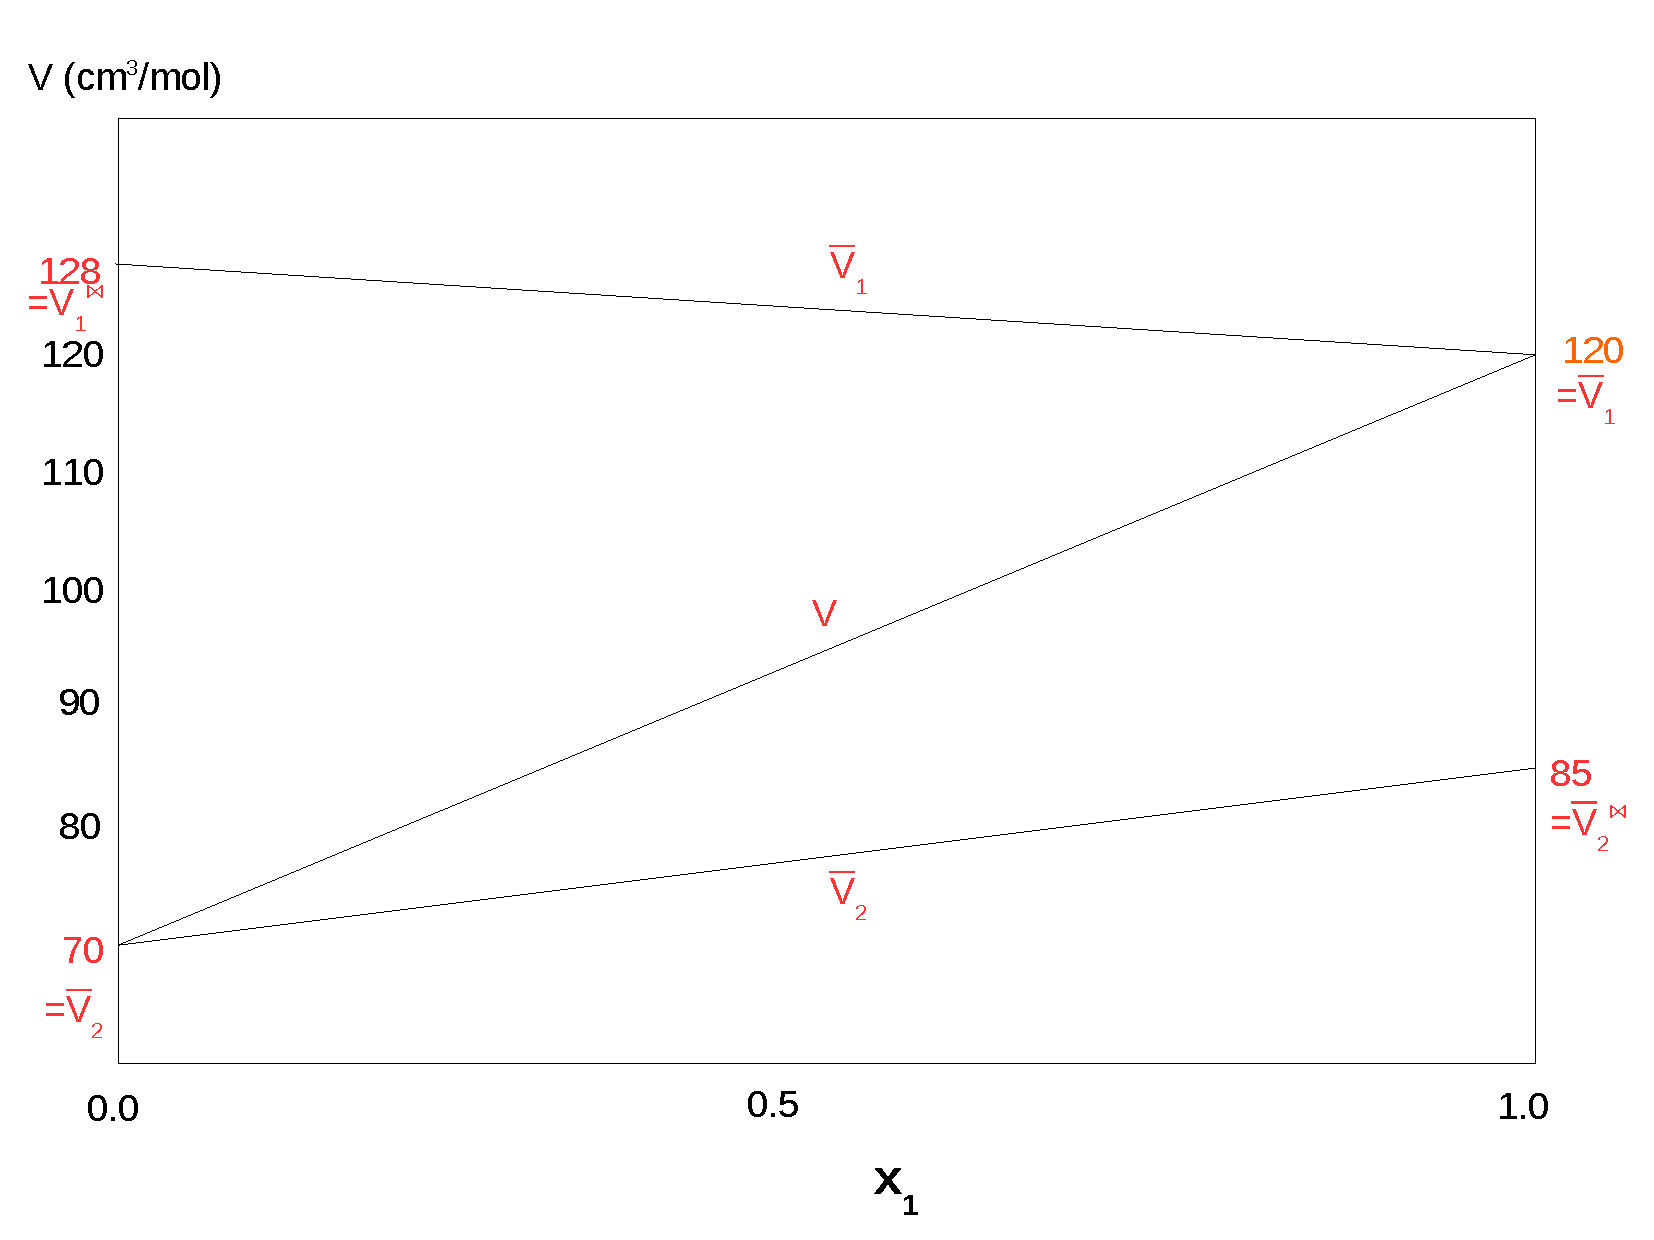
\includegraphics[width=15.cm,height=13.cm,clip]{./Pics/Vxplot}
\end{center}
where~\solmarks{6/8}
\begin{center}
\begin{tabular}{c c c}
\hline
              &  ${\bf x_{1}=0.0}$ & ${\bf x_{1}=1.0}$ \\
\hline
${\bf V}$     &     70            & 120              \\
${\bf \overline{V}_{1}}$ & 128   & 120               \\
${\bf \overline{V}_{2}}$ & 70   & 85               \\
\hline
\end{tabular}
\end{center}
}
%=============
\end{enumerate}
\end{question}


\clearpage


%%%
%%% Question 01_R
%%%
\begin{question}
%
\begin{enumerate}[(a)]

% (Shapiro 2.34) 
\item Air contained in a piston-cylinder system undergoes three consecutive processes,
\begin{itemize} 
\item Process 1--2: Isobaric cooling with P$_{1}$=69 kPa and V$_{1}$=0.11 m$^{3}$;
\item Process 2--3: Isochoric heating with P$_{3}$=345 kPa;
\item Process 3--1: Polytropic expansion, with $PV=$ {\it constant}. %Expansion to the initial state, during which the pressure-volume relationship is $PV=$ {\it constant}.
\end{itemize}  
\begin{enumerate}[(i)]
\item Calculate V$_{2}$ $\left(\text{in m}^{3}\right)$.~\marks{3} 
\solution{
For Process 2--3: V$_{2}$=V$_{3}$. However the expansion 3--1 follows $PV=$ constant,
\begin{displaymath}
P_{1}V_{1}=P_{3}V_{3} \Longrightarrow V_{3} = \frc{P_{1}V_{1}}{P_{3}} = {\bf 0.022\;\text{m}^{3} = V_{2}}
\end{displaymath}~\solmarks{3/3}
}
\item Calculate the work (in $kJ$) for each process.~\marks{6}
\solution{\noindent
Process 1--2: 
\begin{displaymath}
{\bf W_{1-2}} = \int\limits_{V_{1}}^{V_{2}} P dV = P\left(V_{2}-V_{1}\right) = -6072 J \Rightarrow {\bf -6.072 kJ}
\end{displaymath}~\solmarks{2/6}
\noindent
Process 2--3: V$_{2}$=V$_{3}$ $\Longrightarrow$ {\bf W$_{2-3}$ = 0}~\solmarks{2/6} \\
\noindent
Process 3--1: $PV = C$
\begin{displaymath} 
{\bf W_{31}} = \int\limits_{V_{3}}^{V_{1}}P dV = \int\limits_{V_{3}}^{V_{1}}\frc{C}{V} dV = P_{1}V_{1}\ln\frc{V_{1}}{V_{3}} = 12220 J \Rightarrow {\bf 12.22 kJ} 
\end{displaymath}~\solmarks{2/6}
}
\item Sketch the $PV$ diagram for these processes.~\marks{4}
\solution{\solmarks{4/4}
\begin{center}
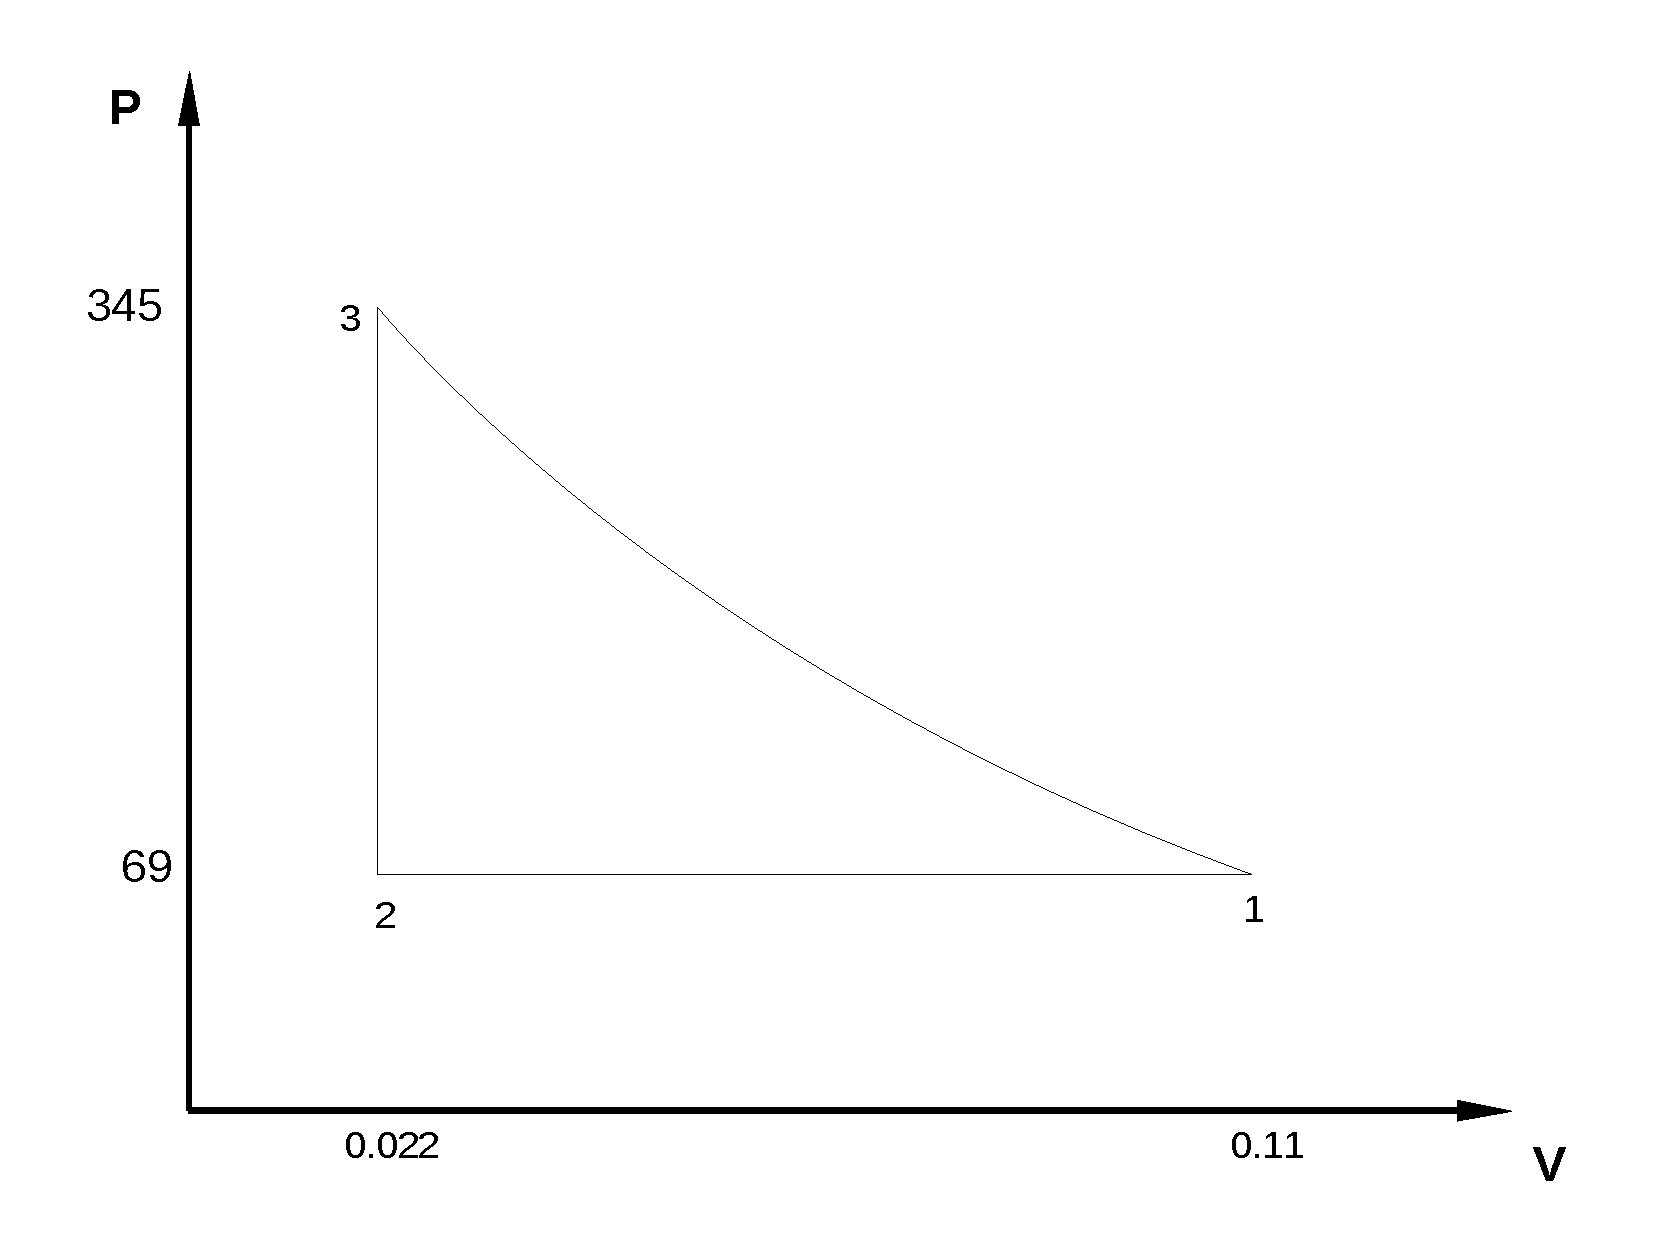
\includegraphics[width=10.cm,height=8.cm,clip]{./Pics/Exam_PV_Diagram}
\end{center}
}
\end{enumerate}

%
\item Calculate the fugacity of steam at 300$^{\circ}$C and 80 bar. For your calculations, you should use $h=$ 2785 kJ/kg, $s=$ 5.791 kJ/(kg.K) for steam at 300$^{\circ}$C and 80 bar. Specific enthalpy and entropy of ideal gas at 300$^{\circ}$C and 0.1 bar are $h^{\text{IG}}=$ 3077 kJ/kg and $s^{\text{IG}}=$ 9.281 kJ/(kg.K), respectively. Assume that,
\begin{displaymath}
 d\mu = dG = RTd\left(\ln{f}\right).
\end{displaymath} 
Also, molar mass of water is 18 g/mol.~\marks{7}

%=======================
\solution{ We can integrate this equation from low pressure so that fugacity is similar to pressure and the system can be considered an ideal gas,\solmarks{2/7}
\begin{displaymath}
\int\limits_{G^{\text{IG}}}^{G}dG = RT\int\limits_{P}^{f}d\left(\ln{f}\right) \Longrightarrow f = P\exp{\left(\frc{G-G^{\text{IG}}}{RT}\right)}
\end{displaymath}
The specific gibbs free energy of ideal gas (at low pressure)~\solmarks{1/7}
\begin{displaymath}
g^{\text{IG}} = h^{\text{IG}}-Ts^{\text{IG}} = -2242.41 kJ/kg \Longrightarrow G^{\text{IG}} = -2242.41 \frc{kJ}{kg} \cdot 18\frc{g}{mol}\cdot\frc{1\; kg}{1000\; g} = -40.36 kJ/mol
\end{displaymath}
Now at 300$^{\circ}$C and 80 bar,~\solmarks{1/7}
\begin{displaymath}
g = h - Ts = -534.11 kJ/kg \Longrightarrow G = -9.61 kJ/mol
\end{displaymath}
Now calculating the fugacity,~\solmarks{3/7}
\begin{displaymath}
f = P\exp{\left(\frc{G-G^{\text{IG}}}{RT}\right)} = 63.47 bar
\end{displaymath}
}
%=======================
%
\end{enumerate}
%
\end{question}
\clearpage

%%%
%%% Question 02_R
%%%
\begin{question}
%
\begin{enumerate}[(a)]
%
\item Develop expressions for the volume expansivity, $\beta=\frc{1}{V}\left(\frc{\partial V}{\partial T}\right)_{P}$, and isothermal compressibility, $\kappa=-\frc{1}{V}\left(\frc{\partial V}{\partial P}\right)_{T}$, for the following equations of state,
\begin{enumerate}[(i)]
\item ideal gas~\marks{4}
\solution{Ideal gas: $V=\frc{RT}{P}$,
\begin{displaymath}
\left(\frc{\partial V}{\partial T}\right)_{P} = \frc{R}{P} \;\;\; \left(\frc{\partial V}{\partial P}\right)_{T} = -\frc{RT}{P^{2}} 
\end{displaymath}~\solmarks{2/4}
Now deriving $\beta$ and $\kappa$,
\begin{displaymath}
{\bf \beta} = \frc{1}{V}\frc{R}{P} {\bf = \frc{1}{T}}\;\;\text{ and}\;\;\kappa = -\frc{1}{V}\left(-\frc{RT}{P^{2}}\right){\bf = \frc{1}{P}}
\end{displaymath}~\solmarks{2/4}
}
\item $V=\frc{RT}{P}+b$~\marks{4}
\solution{
The derivatives are,
\begin{displaymath}
\left(\frc{\partial V}{\partial T}\right)_{P} = \frc{R}{P} \;\;\; \left(\frc{\partial V}{\partial P}\right)_{T} = -\frc{RT}{P^{2}} 
\end{displaymath}~\solmarks{2/4}
Now deriving $\beta$ and $\kappa$,
\begin{displaymath} 
{\bf \beta} = \frc{1}{V}\frc{R}{P} =\frc{R}{V}\frc{V-b}{RT}= {\bf = \frc{1}{T}\frc{V-b}{V}} \;\;\text{ and }\;\; {\bf \kappa} = -\frc{1}{V}\left(-\frc{RT}{P^{2}}\right){\bf = \frc{1}{P}\left[\frc{V-b}{V}\right]}
\end{displaymath}~\solmarks{2/4}
}
\end{enumerate}

\item Calculate the compressibility factor ($Z$) and molar volume of sulphur dioxide $\left(SO_{2}\right)$ vapour at 300 K and 4 bar using the Redlich-Kwong equation of state. Properties of SO$_{2}$ are: T$_{c}$ = 430 K, P$_{c}$ = 78.7 bar and $\omega$ = 0.251 (accentric factor). If you are using an iterative method, do use $Z_{0}=1$ as initial guess of $Z$, and stop at the second iteration $\left(Z_{2}\right)$.~\marks{12}
\solution{ The generic form of $Z$ is,
\begin{displaymath}
Z = 1+ \beta - q\beta\frc{Z - \beta}{\left(Z+\epsilon\beta\right)\left(Z+\sigma\beta\right)}\;\;\text{ with} \;\; \beta = \Omega \frc{P_{r}}{T_{r}}\;\;\text{ and}\;\; q=\frc{\Psi\alpha}{\Omega T_{r}}
\end{displaymath}
For SRK with {\bf T$_{r}$=0.8380}, {\bf P$_{r}$=0.3754}, {\bf $\beta$=3.88$\times$10$^{-2}$} and {\bf $q$=6.7274}~\solmarks{2/12},
\begin{displaymath}
{\bf Z = 1 + \beta - q\beta\frc{Z-\beta}{Z^{2}+\beta Z}}
\end{displaymath}~\solmarks{2/12}
The equation is non-linear and to find the root we can apply Newton-Raphson method 
\begin{displaymath}
Z_{i} = Z_{i-1} - \frc{\mathcal{F}\left(Z_{i-1}\right)}{d\mathcal{F}/dZ \left(Z_{i-1}\right)}
\end{displaymath}
with,
\begin{eqnarray}
&& \mathcal{F}\left(Z\right) = Z - \left[ 1 + \beta - q\beta\frc{Z-\beta}{Z^{2}+\beta Z}\right] \nonumber \\
&& \frc{d\mathcal{F}}{dZ}\left(Z\right) = 1 + q\beta \frc{\beta^{2}+2\beta Z- Z^{2}}{\left(Z^{2}+\beta Z\right)^{2}} \nonumber
%\frc{q\beta\left(Z^{2}\beta +Z\right)-q\beta Z\left(2Z + \beta\right)}{\left(Z^{2}+\beta Z\right)^{2}} + \frc{q\beta^{2}\left(2Z+\beta\right)}{\left(Z^{2}+\beta Z\right)^{2}} \nonumber
\end{eqnarray} 
as initial guess, we can use the generic real gas EOS, $PV=Z_{0}RT \Longrightarrow$ {\bf $Z_{0}=0.7217$}~\solmarks{2/12}. Thus 
\begin{center}
{\bf $Z_{1}$ = 0.7184}~\solmarks{3/12} \\
{\bf $Z_{2}$ = 0.7160}~\solmarks{3/12} \\
$\cdots \cdots \cdots $ \\
\textcolor{red} {or (using calculator) }{\bf $Z_{22}$ = 0.7088}~\solmarks{\textcolor{red}{8/12}} \\

\end{center}
} 
%
\end{enumerate}
%
\end{question}

\clearpage

%%%
%%% Question 03_R
%%%
\begin{question}
%
\begin{enumerate}[(a)]
%%%
%%% Johannes T0902
%%%
\item\label{T0902} Assuming that all species and their mixtures are ideal gases, derive an equation for the Gibbs energy as a function of the reaction coordinate for the reaction below at 1000K.
\begin{displaymath}
H_{2} + CO_{2} \Longleftrightarrow H_{2}O + CO
\end{displaymath}
Calculate the reaction coordinate, $\epsilon$, in the equilibrium.
Given $\Delta G_{f}^{\circ}$ $\left(\text{kJ.mol}^{-1}\right)$ at 1000K: (a) H$_{2}$O: -192.42, (b) CO: -200.24 and (c) CO$_{2}$: -395.79.~\marks{13}

%==========================
\solution{ The Gibbs energy can be expressed as~\solmarks{1/13}
\begin{eqnarray}
G &=& \sum y_{i}G_{i} + RT\sum y_{i}\ln{y_{i}} \nonumber \\
G &=& \sum y_{i}\Delta G^{o}_{f,i} + RT\sum y_{i}\ln{y_{i}} \nonumber 
\end{eqnarray}
We can differentiate the total Gibbs energy as,
\begin{displaymath}
dG^{t} = d\left(n G\right) = n\frc{dG}{d\epsilon} + G\frc{d n}{d\epsilon} 
\end{displaymath} 
Assuming the system is closed and in equilibrium: $dn = 0$ and $\frc{dG}{d\epsilon}=0$. For 1 mole of H$_{2}$ and CO$_{2}$, the mole fraction of the gaseous species are~\solmarks{1/13}
\begin{displaymath}
y_{\text{H}_{2}}=\frc{1-\epsilon}{2} =y_{\text{CO}_{2}}\;\;\text{ and }\;\; y_{\text{H}_{2}\text{O}}=\frc{\epsilon}{2} =y_{\text{CO}}\
\end{displaymath}
Thus,~\solmarks{5/13}
\begin{eqnarray}
 G &=& \left(y_{H_{2}}\Delta G^{o}_{f,H_{2}} + y_{CO_{2}}\Delta G^{o}_{f,CO_{2}} + y_{H_{2}O}\Delta G^{o}_{f,H_{2}O} + y_{CO}\Delta G^{o}_{f,CO}\right) + \nonumber \\
    && RT\left(y_{H_{2}}\ln{y_{H_{2}}} + y_{CO_{2}}\ln{y_{CO_{2}}} + y_{H_{2}O}\ln{y_{H_{2}O}} + y_{CO}\ln{y_{CO}}\right) \nonumber \\
   &=&\left[\frc{1-\epsilon}{2}\Delta G^{o}_{f,CO_{2}} + \frc{\epsilon}{2}\left(\Delta G^{o}_{f,H_{2}O}+\Delta G^{o}_{f,CO}\right)\right] + RT\left[\left(1-\epsilon\right)\ln{\frc{1-\epsilon}{2}} + \epsilon\ln{\frc{\epsilon}{2}}\right]\nonumber
\end{eqnarray}
for $\Delta G^{o}_{f,H_{2}} = 0$. In the equilibrium $\frc{dG}{d\epsilon}=0$~\solmarks{1/13}, therefore~\solmarks{5/13}
\begin{displaymath}
\frc{dG}{d\epsilon} = B-A + RT\left[\ln{\frc{\epsilon}{2}} - \ln{\frc{1-\epsilon}{2}}\right] = 0 \Longrightarrow \epsilon = 0.4531 
\end{displaymath}
with $A=\frc{-395790}{2}$ and $B=\frc{-192420-200240}{2}$.
}
%==========================
%

%%%
%%% Problem 8.3 (Power Lectures Notes)
%%%
\item Saturated ammonia $\left(\text{NH}_{3}\right)$ vapour at $P_{1} = 200$ kPa is compressed by a piston to $P_{2} = 1.6$ MPa in a reversible adiabatic process. Calculate the work done per unit mass.~\marks{7}

%=========================
\solution{At 200 kPa (2 bar), from the saturated tables:~\solmarks{2/7}
\begin{center}
\begin{tabular}{c c } 
 $v_{1}=0.5946\;m^{3}/kg$ &$T_{1}=-18.86^{\circ}C$ \\
 $s_{1}=5.5969\;kJ/(kg.K)$ & $u_{1}=1300.39\;kJ/kg$\\
\end{tabular}
\end{center}
Reversible and adiabatic compresion implied in isentropic process, therefore $s_{2}=s_{1}$. At  $P_{2}=1.6\text{ MPa}=16\text{ bar}$, the specific entropy of saturated ammonia vapour is 4.8542 kJ/(kg.K), which is smaller than $s_{1}$, indicating that the fluid is at superheated state. With $P_{2}$ and $s_{2}$, in the superheated fluid table we can obtain (through linear interpolation),~\solmarks{2/7}
\begin{center}
\begin{tabular}{c c } 
 $v_{2}=0.1180\;m^{3}/kg$ &$T_{2}=135.16^{\circ}C$ \\
 $s_{2}=5.5969\;kJ/(kg.K)$ & $u_{2}=1546.50\;kJ/kg$\\
\end{tabular}
\end{center}
From the First Law,~\solmarks{3/7}
\begin{eqnarray}
   && \Delta u = q + w \text{ with } q=0 \text{ because the process is adiabatic} \nonumber \\
   && w = u_{2}-u_{1} = 246.11 \text{kJ/kg (positive because work is given to the system).}\nonumber
\end{eqnarray}


}
%=========================


\end{enumerate}
%
\end{question}

\clearpage

%%%
%%% Question 04_R
%%%
\begin{question}

 Estimate the bubble and dew point temperatures of a 25 mol$\%$ n-pentane $\left(nC_{5}\right)$, 45 mol$\%$ n-hexane $\left(nC_{6}\right)$ and 30 mol$\%$ n-heptane $\left(nC_{7}\right)$ mixture at 1.013 bar. Also calculate the compositions at dew and bubble points. ~\marks{20}
%\solution{ iouh}

For this problem, use 
\begin{displaymath}
   \ln P_{i}^{\text{sat}} = A_{i} - \frc{B_{i}}{RT}
\end{displaymath} 
with [P] = bar, [T] = K, $\left[\text{B}_{i}\right]$ = J/mol and
    \begin{center}
       \begin{tabular}{l l l} 
          $A_{nC_{5}}=10.422$ & $A_{nC_{6}}=10.456$ & $A_{nC_{7}}=11.431$ \\
          $B_{nC_{5}}=26799$  & $B_{nC_{6}}=29676$  & $B_{nC_{7}}=35200$  
       \end{tabular}
    \end{center}
If you are using an iterative method to solve this problem, do stop at the 5$^{th}$ iteration.

%=======================
\solution{For the bubble point, we need to solve~\solmarks{2/20}
\begin{displaymath}
\sum\limits_{i=1}^{3} y_{i} = 1 = \frc{x_{C5}P_{C5}^{sat}}{P} + \frc{x_{C6}P_{C6}^{sat}}{P} + \frc{x_{C7}P_{C7}^{sat}}{P}  
\end{displaymath}
for $T$, with 
\begin{displaymath}
   \ln P_{i}^{\text{sat}} = A_{i} - \frc{B_{i}}{RT}.
\end{displaymath} 
Leading to $T=334.94$ K (at the 5$^{th}$ iteration)~\solmarks{5/20} with composition $y = \left[0.5483\; 0.0883\; 0.3634\right]$ for n-pentane, n-hexane and n-heptane, respectively.~\solmarks{3/20}.

For the dew point, we need to  solve~\solmarks{2/20}
\begin{displaymath}
\sum\limits_{i=1}^{3} x_{i} = 1 = \frc{y_{C5}P}{P_{C5}^{sat}} + \frc{y_{C6}P}{P_{C6}^{sat}} + \frc{y_{C7}P}{P_{C7}^{sat}}  
\end{displaymath}
for $T$, leading to $T=350.58$ K (at the 5$^{th}$ iteration)~\solmarks{5/20} with composition $x = \left[0.0742\; 0.3463\; 0.5795\right]$.~\solmarks{3/20}

}
%=======================
%
\end{question}

\clearpage

%%%
%%% Question 05_R
%%%
\begin{question}
%
\begin{enumerate}[(a)]

%%% Johannes T0602
%%%
\item\label{T0602} What is the change in entropy when 700 litres of CO$_{2}$ and 300 litres of N$_{2}$ form a gas mixture at 1 bar and 25$^{\circ}$C? Assume ideal gases, and given
\begin{displaymath}
\Delta S = - nR\sum\limits_{i=1}^{n}y_{i}\ln{y_{i}},
\end{displaymath}
where $S$, $n$ and $y$ are entropy, number of moles and mole fraction, respectively.~\marks{10}

%===========================
\solution{ For CO$_{2}$ (1) and N$_{2}$ (2) at 1 bar and 25$^{\circ}$C with ideal gas behaviour, {\it mole fraction (x$_{i}$) = volume fraction (y$_{i}$)} as,~\solmarks{2/10}
\begin{eqnarray}
 &&x_{i} = \frc{n_{i}}{n}, \text{ and }  y_{i}=\frc{V_{i}}{V} \nonumber \\
 && x_{i} = \frc{n_{i}}{n} = \frc{PV_{i}/(RT)}{PV/(RT)} = \frc{V_{i}}{V} \nonumber 
\end{eqnarray}
Therefore,~\solmarks{2/10}
\begin{eqnarray}
y_{1} = 0.7 \;\;\Longrightarrow V_{1}^{t} = 0.7\;cm^{3} \nonumber \\
y_{2} = 0.3 \;\;\Longrightarrow V_{2}^{t} = 0.3\;cm^{3} \nonumber
\end{eqnarray}
At $P=1$ bar and $T=298.15$ K, the number of moles, $n$, is~\solmarks{2/10}
\begin{displaymath}
n = \frc{P}{RT}\sum V_{i}^{t} = 40.34 \text{moles}
\end{displaymath}
The entropy change is~\solmarks{4/10}
\begin{displaymath}
\Delta S = - nR\sum\limits_{i=1}^{n}y_{i}\ln{y_{i}} = 204.88\text{ J/K}
\end{displaymath}

}
%===========================


%%%
%%% Nguyen (pg 128, Ex 5.3-1)
%%%
\item Calculate the bubble point pressure and vapour composition for a liquid mixture of 41.2 mol$\%$ of ethanol (1) and n-hexane (2) at 331 K. Given,
\begin{eqnarray}
&& \ln{\gamma_{1}} = \frc{A}{\left(1+\frc{Ax_{1}}{Bx_{2}}\right)^{2}},\;\;\ln{\gamma_{2}} = \frc{A}{\left(1+\frc{Bx_{2}}{Ax_{1}}\right)^{2}} \nonumber \\
&& \ln{P_{1}^{sat}} = C_{1} + \frc{D_{1}}{T+E_{1}},\;\; \ln{P_{2}^{sat}} = C_{2} + \frc{D_{2}}{T+E_{2}} \nonumber 
\end{eqnarray}
where $A=$ 2.409, $B=$ 1.970, $C_{1}$ = 16.1952, $C_{2}=$ 14.0568, $D_{1}=$ -3423.53, $D_{2}=$ -2825.42, $E_{1}=$ -55.7152, $E_{2}=$ -42.7089. [P] = kPa and [T] = $\left[\text{D}_{i}\right]$ = $\left[\text{E}_{i}\right]$ = K.~\marks{10}

%========================
\solution{ At 331 K, the saturation pressures are $P_{1}^{sat}=$ 42.90 kPa and $P_{2}^{sat}=$ 7054 kPa.~\solmarks{2/10}

The liquid solution with $x_{1}=0.412$ and $x_{2}=0.588$ results in the following activity coefficient $\gamma_{1}=2.011$ and $\gamma_{2}=1.521$.~\solmarks{2/10}

The partial pressure of ethanol and n-hexane are,~\solmarks{2/10}
\begin{eqnarray}
P_{1} = x_{1}\gamma_{1}P_{1}^{sat} = 35.55\text{ kPa} \nonumber \\
P_{2} = x_{2}\gamma_{2}P_{2}^{sat} = 63.09\text{ kPa} \nonumber 
\end{eqnarray}
The bubble pressure is~\solmarks{2/10}
\begin{displaymath}
P =P_{1} + P_{2} = 98.64\text{ kPa}
\end{displaymath}
And the composition of the vapour phase is~\solmarks{2/10}
\begin{displaymath}
y_{1} = \frc{P_{1}}{P} = 0.360\;\;\text{ and } \;\; y_{2} = 0.640
\end{displaymath}

}
%========================

\end{enumerate}
\end{question}

\clearpage

%%%
%%% Question 07
%%%
\begin{question}
%
\begin{enumerate}[(a)]
% Nguyen pg.5-25
\item Calculate the bubble point pressure and vapour composition for a liquid mixture of 41.2 mol$\%$ ethanol (1) and n-hexane (2) at 331K. Given:
\begin{displaymath}
\ln{\gamma_{1}} = \frac{A}{\left[1+\left(Ax_{1} / Bx_{2}\right)\right]^{2}} \;\;\text{ and }\;\; \ln{\gamma_{2}} = \frac{B}{\left[1+\left(Bx_{2} / Ax_{1}\right)\right]^{2}}
\end{displaymath}
with $A=2.409$ and $B=1.970$. Also,
\begin{displaymath}
\ln{P_{1}^{\text{sat}}} = 16.1952 - \frac{3423.53}{T-55.7152} \;\;\text{ and }\;\; \ln{P_{2}^{\text{sat}}} = 14.0568 - \frac{1825.42}{T-42.7089}
\end{displaymath}
with $P_{i}^{\text{sat}}$ in $kPa$ and $T$ in $K$ 


\end{enumerate}
\end{question}

\clearpage

%%%%%%%%%%%%%%%%%%%%%%%%%%%%%%%%%%%%%%%%%%%%%%%%%%%%%%%%%%%%%%%%%%%%%%%%%%%%%%%%%%%%%%%%%%
%%%%                                                                                  %%%%
%%%%                                     2014-15                                      %%%%  
%%%%                                                                                  %%%% 
%%%%%%%%%%%%%%%%%%%%%%%%%%%%%%%%%%%%%%%%%%%%%%%%%%%%%%%%%%%%%%%%%%%%%%%%%%%%%%%%%%%%%%%%%%

\begin{center}
\Huge{Exams 2014-15}
\end{center}

\clearpage

%%%
%%% Question 01
%%%
\begin{question}
%
\begin{enumerate}[(a)] % (Shapiro 2.34) 
\item A closed system with 0.09 kg of air undergoes a polytropic process from P$_{1}$ = 138 kPa, v$_{1}$=0.72 m$^{3}$.kg$^{-1}$ to a final state where P$_{2}$ = 552 kPa, v$_{2}$ = 0.25 m$^{3}$.kg$^{-1}$.  Determine the work (in $kJ$) required for this compression.~\marks{8} 
\solution{
First stage is to calculate the polytropic coefficient,
\begin{displaymath}
P_{1}v_{1}^{n} = P_{2}v_{2}^{n} \Longrightarrow {\bf n} = \frc{\ln P_{2}/P_{1}}{\ln v_{1}/v_{2}} {\bf = 1.31}
\end{displaymath}~\solmarks{4/8}
Now, calculating the work with $V_{i}=v_{i}\times m$, thus V$_{1}=0.0648$ m$^{3}$ and V$_{2}=0.0225$ m$^{3}$:
\begin{eqnarray}
{\bf W }&=& \int\limits_{V_{1}}^{V_{2}} P dV = \int\limits_{V_{1}}^{V_{2}} \frc{C}{V^{n}} dV = \left.C \frc{V^{1-n}}{1-n}\right|_{V_{1}}^{V_{2}} = \frc{P_{2}V_{2}^{n}V_{2}^{1-n}-P_{1}V_{1}^{n}V_{1}^{1-n}}{1-n} = \frc{P_{2}V_{2}-P_{1}V_{1}}{1-n} \nonumber \\
   &=& {\bf -11.214 kJ} \nonumber
\end{eqnarray} ~\solmarks{4/8}}



\item Calculate the compressibility factor ($Z$) of chloroform vapour at 450 K and 20 bar (molar volume of 1.35$\times$10$\left.^{-3}\text{ m}^{3}.\text{gmol}^{-1}\right)$ using the Soave-Redlich-Kwong equation of state. Properties of chloroform are: T$_{c}$ = 537 K, P$_{c}$ = 5328.68 kPa and $\omega$ =0.218 (accentric factor). In your iterative calculations, use $PV=ZRT$ as an initial guess of $Z$, and stop at the second iteration $\left(Z_{2}\right)$.~\marks{12}
\solution{ The generic form of $Z$ is,
\begin{displaymath}
Z = 1+ \beta - q\beta\frc{Z - \beta}{\left(Z+\epsilon\beta\right)\left(Z+\sigma\beta\right)}\;\;\text{ with} \;\; \beta = \Omega \frc{P_{r}}{T_{r}}\;\;\text{ and}\;\; q=\frc{\Psi\alpha}{\Omega T_{r}}
\end{displaymath}
For SRK with {\bf T$_{r}$=0.8380}, {\bf P$_{r}$=0.3754}, {\bf $\beta$=3.88$\times$10$^{-2}$} and {\bf $q$=6.7274}~\solmarks{2/12},
\begin{displaymath}
{\bf Z = 1 + \beta - q\beta\frc{Z-\beta}{Z^{2}+\beta Z}}
\end{displaymath}~\solmarks{2/12}
The equation is non-linear and to find the root we can apply Newton-Raphson method 
\begin{displaymath}
Z_{i} = Z_{i-1} - \frc{\mathcal{F}\left(Z_{i-1}\right)}{d\mathcal{F}/dZ \left(Z_{i-1}\right)}
\end{displaymath}
with,
\begin{eqnarray}
&& \mathcal{F}\left(Z\right) = Z - \left[ 1 + \beta - q\beta\frc{Z-\beta}{Z^{2}+\beta Z}\right] \nonumber \\
&& \frc{d\mathcal{F}}{dZ}\left(Z\right) = 1 + q\beta \frc{\beta^{2}+2\beta Z- Z^{2}}{\left(Z^{2}+\beta Z\right)^{2}} \nonumber
%\frc{q\beta\left(Z^{2}\beta +Z\right)-q\beta Z\left(2Z + \beta\right)}{\left(Z^{2}+\beta Z\right)^{2}} + \frc{q\beta^{2}\left(2Z+\beta\right)}{\left(Z^{2}+\beta Z\right)^{2}} \nonumber
\end{eqnarray} 
as initial guess, we can use the generic real gas EOS, $PV=Z_{0}RT \Longrightarrow$ {\bf $Z_{0}=0.7217$}~\solmarks{2/12}. Thus 
\begin{center}
{\bf $Z_{1}$ = 0.7184}~\solmarks{3/12} \\
{\bf $Z_{2}$ = 0.7160}~\solmarks{3/12} \\
$\cdots \cdots \cdots $ \\
\textcolor{red} {or (using calculator) }{\bf $Z_{22}$ = 0.7088}~\solmarks{\textcolor{red}{8/12}} \\

\end{center}
} 

\end{enumerate}

\end{question} 
\clearpage

%%%
%%% Question 02
%%%
\begin{question}
%
A geothermal power station (Rankine cycle) uses propane $\left(\text{n-C}_{3}\right)$ as working fluid to produce power $\left(W_{T}\right)$ in a turbine (isentropic expansion) with efficiency $\left(\eta_{T}\right)$ of 90$\%$. n-C$_{3}$ is vaporised by geothermal water (brine, $A-B$ in the diagram) at 90$^{\circ}$C. After condensed, n-C$_{3}$ is driven to a heat exchanger (with thermal efficiency of 68$\%$) and the cycle continues. The mass flow rate of n-C$_{3}$ $\left(\dot{m}_{C3}\right)$ is 250 kg.s$^{-1}$ and the heat capacity at constant pressure $\left(C_{p}\right)$ of brine is 3565.5 J.(kg.K)$^{-1}$. Conditions for n-C$_{3}$ and brine flows are described in Table below.
%\vspace{-.9cm}
\begin{center}
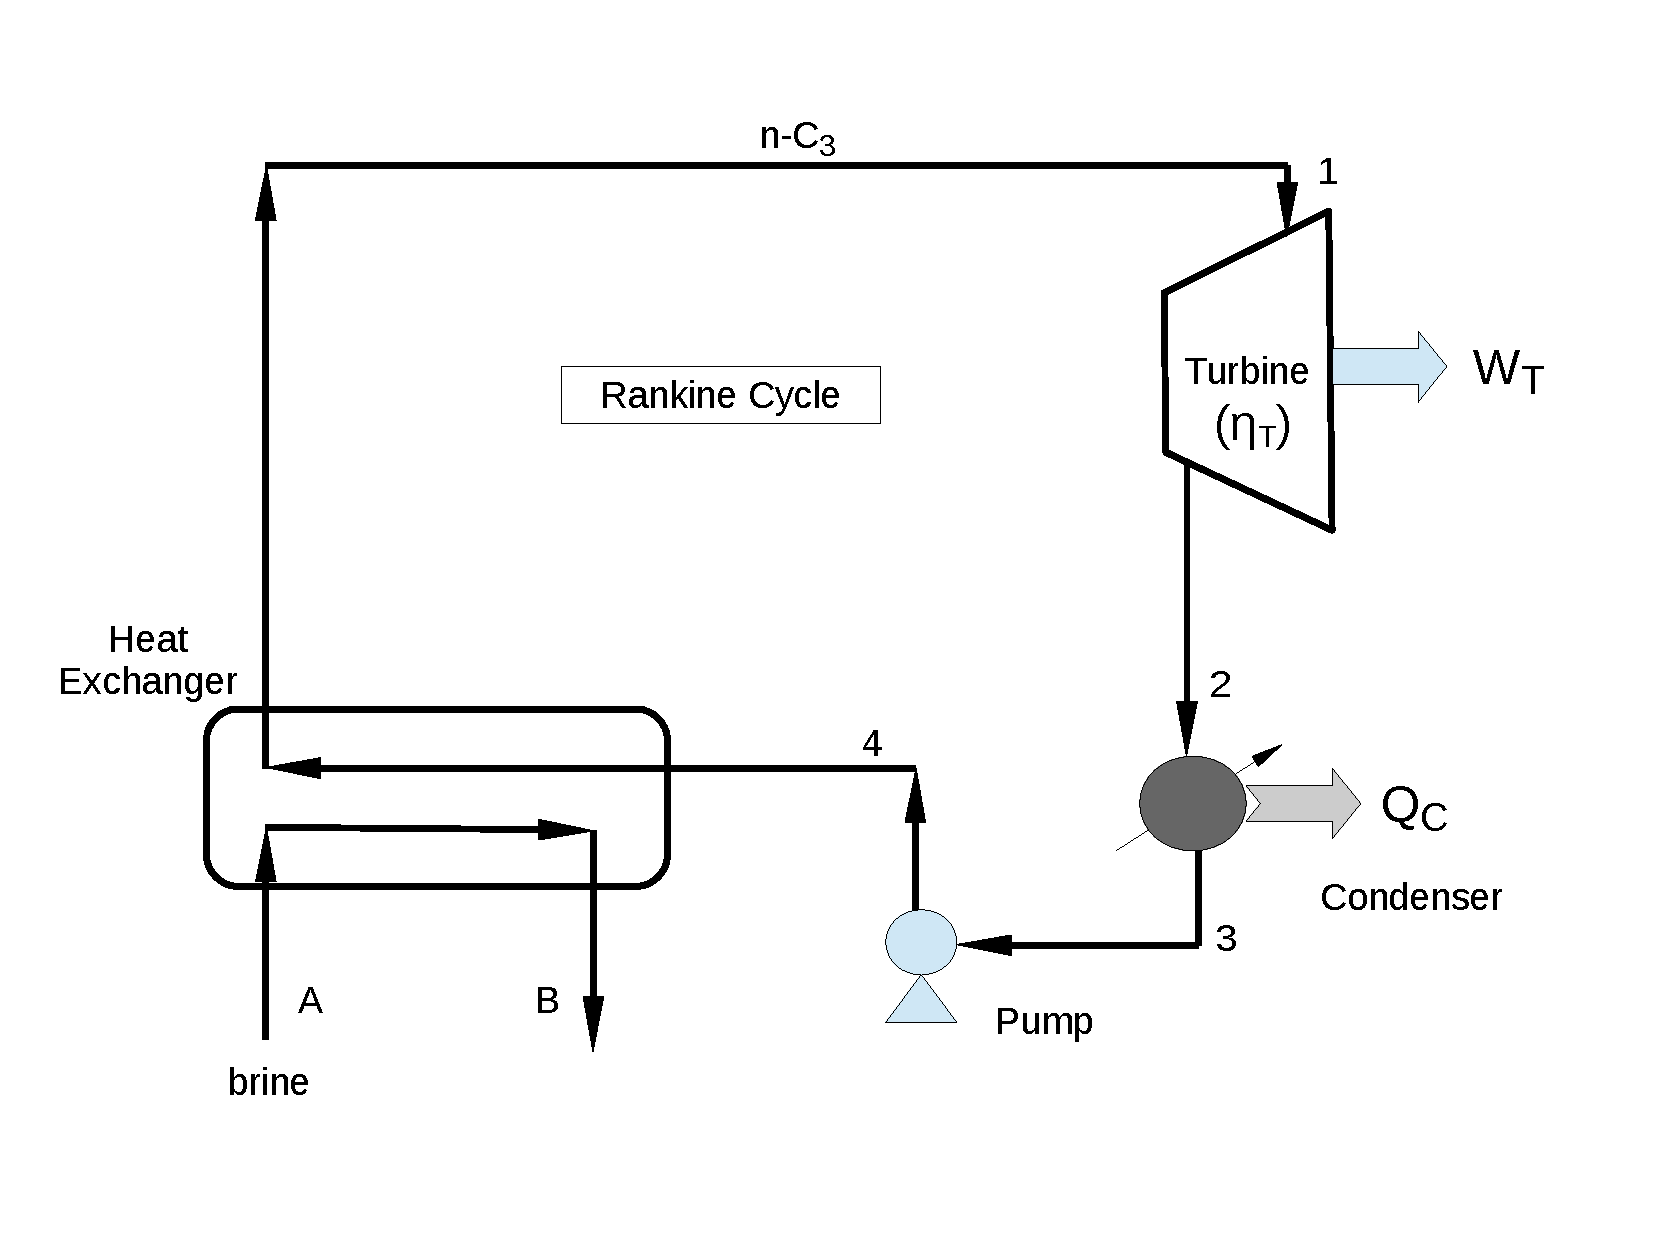
\includegraphics[width=10.cm,height=7.cm,clip]{./Pics/RankineCycle}
%\caption{ Reheat and regenerative Rankine cycle with 2 turbines.}
%\label{exam_mod02_rankinecycle}
\end{center}
%\vspace{-1.5cm}
\begin{center}
\begin{tabular} {||c | c c c c c || }
\hline\hline
{\bf Stage} & {\bf P}    & {\bf T}        & {\bf State}    & {\bf H}             & {\bf S}                  \\
            & {\bf (bar)}& {\bf ($^{o}$C)} &               & {\bf (kJ.kg$^{-1}$)} & {\bf (kJ.(kg.K)$^{-1}$)}  \\
\hline\hline
 {\bf 1 }   & 16         & 50             &   {\bf (a)}    & {\bf (b)}           & {\bf (c)}                \\
 {\bf 2 }   & 6          &  --            &   wet vapour   & {\bf (d)}           & --                       \\
 {\bf 3 }   & 6          &                &   sat. liquid  & {\bf (e)}           & --                       \\
 {\bf 4 }   & 16         &                &   {\bf (f)}    & {\bf (g)}           & --                       \\
 {\bf A }   & --         & 90             &   --           & --                  & --                       \\
 {\bf B }   & --         & 30             &   --           & --                  & --                       \\
 \hline\hline
\end{tabular}
\end{center}

\begin{enumerate}[(a)]
%%
%% Question A
%%
\item In this Table, determine {\it (a)-(g)}.~\marks{7}
%
\solution{
In order to fill the Table we need to calculate the thermodynamic properties for each stage of the cycle:
\begin{description}
%%%
\item[Stage 1:] At P$_{1}$ = 16 bar, T$_{1}$ = 50$^{\circ}$C $>$ T$_{sat}\left(P_{1}\right)$ = 46.89$^{\circ}$C. Therefore the fluid is at {\bf superheated state}~\solmarks{1/7}. From the superheated table for n-C$_{3}$ at P$_{1}$ and T$_{1}$, we can obtain:\\
{\bf H$_{1}$ = 522.5 kJ.kg$^{-1}$}~\solmarks{1/7} and\\
{\bf S$_{1}$ = 1.733 kJ.(kg.K)$^{-1}$}~\solmarks{1/7}. 
%%%
\item[Stage 2:] At P$_{2}$ = 6 bar, the fluid is wet vapour after the isentropic expansion. We should first calculate the quality of the vapour in an ideal expansion (using values of entropy/enthapy obtained from the saturated n-C$_{3}$ table at P$_{2}$.
\begin{displaymath}
x_{2s} =\frc{S_{2s}-S_{f}}{S_{g}-S_{f}} = \frc{1.733 - 0.446}{1.737-0.446} = 0.9969
\end{displaymath}
now to calculate the ideal enthalpy,
\begin{displaymath}
x_{2s} = 0.9969 = \frc{H_{2s}-H_{f}}{H_{g}-H_{f}} = \frc{H_{2s}-115.3}{478.3-115.3}\;\;\Longleftrightarrow\;\; H_{2s} = 477.17 \frc{kJ}{kg}
\end{displaymath}
As the efficiency of the turbine is of 90$\%$,
\begin{displaymath}
\eta_{\text{Turbine}} = 0.90 =\frc{H_{2}-H_{1}}{H_{2s}-H_{1}} = \frc{H_{2} - 522.5}{477.17 - 522.5} \;\;\Longleftrightarrow \;\; {\bf H_{2} = 481.70\frc{kJ}{kg}}
\end{displaymath}~\solmarks{1/7}
%%%
\item[Stage 3:] At P$_{3}$ = P$_{2}$ = 6 bar, the fluid leaving the condenser towards the pump is saturated liquid, and the enthalpy and specific volume are the same of the liquid phase obtained from the saturated table:\\
{\bf H$_{3}$} = H$_{f}\left(\text{P = 6 bar}\right)$ {\bf = 115.3 kJ.kg$^{-1}$}~\solmarks{1/7} \\
V$_{3}$ = V$_{f}\left(\text{P = 6 bar}\right)$ = 1.931$\times$10$^{-3}$ m$^{3}$.kg$^{-1}$ 
%%%
\item[Stage 4:] The fluid leaving the pump is {\bf sub-cooled liquid}.~\solmarks{1/7} As there is no heat loss in the pump, we can assume $dH \approx VdP$, therefore
\begin{displaymath}
{\bf H_{4}} = H_{3} + V_{3}\left(P_{4}-P_{3}\right) = 115.3\frc{kJ}{kg} + 1.931\times 10^{-3} \frc{m^{3}}{kg} \left(16 - 6\right)\text{bar} {\bf= 117.23 \frc{kJ}{kg}}
\end{displaymath}~\solmarks{1/7}

\end{description}
Thus the Table becomes:
\begin{center}
\begin{tabular} {||c | c c c c c || }
\hline\hline
{\bf Stage} & {\bf P}    & {\bf T}        & {\bf State}    & {\bf H}             & {\bf S}                  \\
            & {\bf (bar)}& {\bf ($^{o}$C)} &               & {\bf (kJ.kg$^{-1}$)} & {\bf (kJ.(kg.K)$^{-1}$)}  \\
\hline\hline
 {\bf 1 }   & 16         & 50             &{\bf superheated vapour}&{\bf 522.5}  & {\bf 1.733}              \\
 {\bf 2 }   & 6          &  --            &   wet vapour   & {\bf 481.70}        & --                       \\
 {\bf 3 }   & 6          &                &   sat. liquid  & {\bf 115.3}         & --                       \\
 {\bf 4 }   & 16         &                &{\bf sub-cooled liquid}& {\bf 117.23} & --                       \\
 {\bf A }   & --         & 90             &   --           & --                  & --                       \\
 {\bf B }   & --         & 30             &   --           & --                  & --                       \\
 \hline\hline
\end{tabular}
\end{center}
}
%%
%% Question B
%%
\item Calculate the power produced by the turbine $\left(W_{T}\right)$ and the heat extracted in the condenser $\left(Q_{C}\right)$ in {\it MW}.~\marks{4}
%
\solution{
\begin{displaymath}
{\bf W_{T}} = \dot{m}_{C3} \left(H_{1}-H_{2}\right) = 250\frc{kg}{s} \times \left(522.5 - 481.70\right)\frc{kJ}{kg} = 10200 \frc{kJ}{s} {\bf = 10.2 MW}
\end{displaymath}~\solmarks{2/4}

\begin{displaymath}
{\bf Q_{C}} = \dot{m}_{C3} \left(H_{2}-H_{3}\right) = 250\frc{kg}{s} \times \left(481.70 - 115.30\right)\frc{kJ}{kg} = 91600 \frc{kJ}{s} {\bf = 91.6 MW}
\end{displaymath}~\solmarks{2/4}
} 
%%
%% Question C
%%
\item Calculate the mass flow rate of brine in {\it kg.s}$^{-1}$.~\marks{6}
%
\solution{
The heat extracted by the n-C$_{3}$ $\left(\dot{Q}_{C3}\right)$ fluid in the heat exchanger can be easily calculated by
\begin{displaymath}
{\bf \dot{Q}_{C3}} = \dot{m}_{C3}\left(H_{1}-H_{4}\right) {\bf = 101317.5\frc{kJ}{s}}
\end{displaymath}~\solmarks{2/6}
Assuming that the heat extracted from the geothermal fluid (brine), $\dot{Q}_{gf}$ is transferred to the n-C$_{3}$ stream with efficiency of 68$\%$,
\begin{displaymath}
\eta_{\text{HE}} = 0.68 = \frc{\dot{Q}_{C3}}{\dot{Q_{gf}}} \;\; \Longleftrightarrow  {\bf \dot{Q}_{gf} = 148996.32 \frc{kJ}{s}}
\end{displaymath}~\solmarks{2/6}
With the heat generated by the geothermal fluid and the inlet/outlet fluid temperatures, we can now calculate the brine mass flow rate for the associated heat transferred,
\begin{displaymath} 
\dot{Q}_{gf} = 148996.32 \frc{kJ}{s} = \dot{m}_{gf} C_{p} \left(T_{A} - T_{B}\right)  \;\;\Longleftrightarrow\;\; {\bf \dot{m}_{gf} = 696.57\frc{kg}{s}}
\end{displaymath}~\solmarks{2/6}
}
%%%
%%% Question D
%%%
\item Sketch the temperature $\times$ entropy (TS) diagram for the process indicating the liquid and vapour saturated lines and each stage of the n-C$_{3}$ Rankine cycle.~\marks{3}
%
\solution{~\solmarks{3/3}
\begin{center}
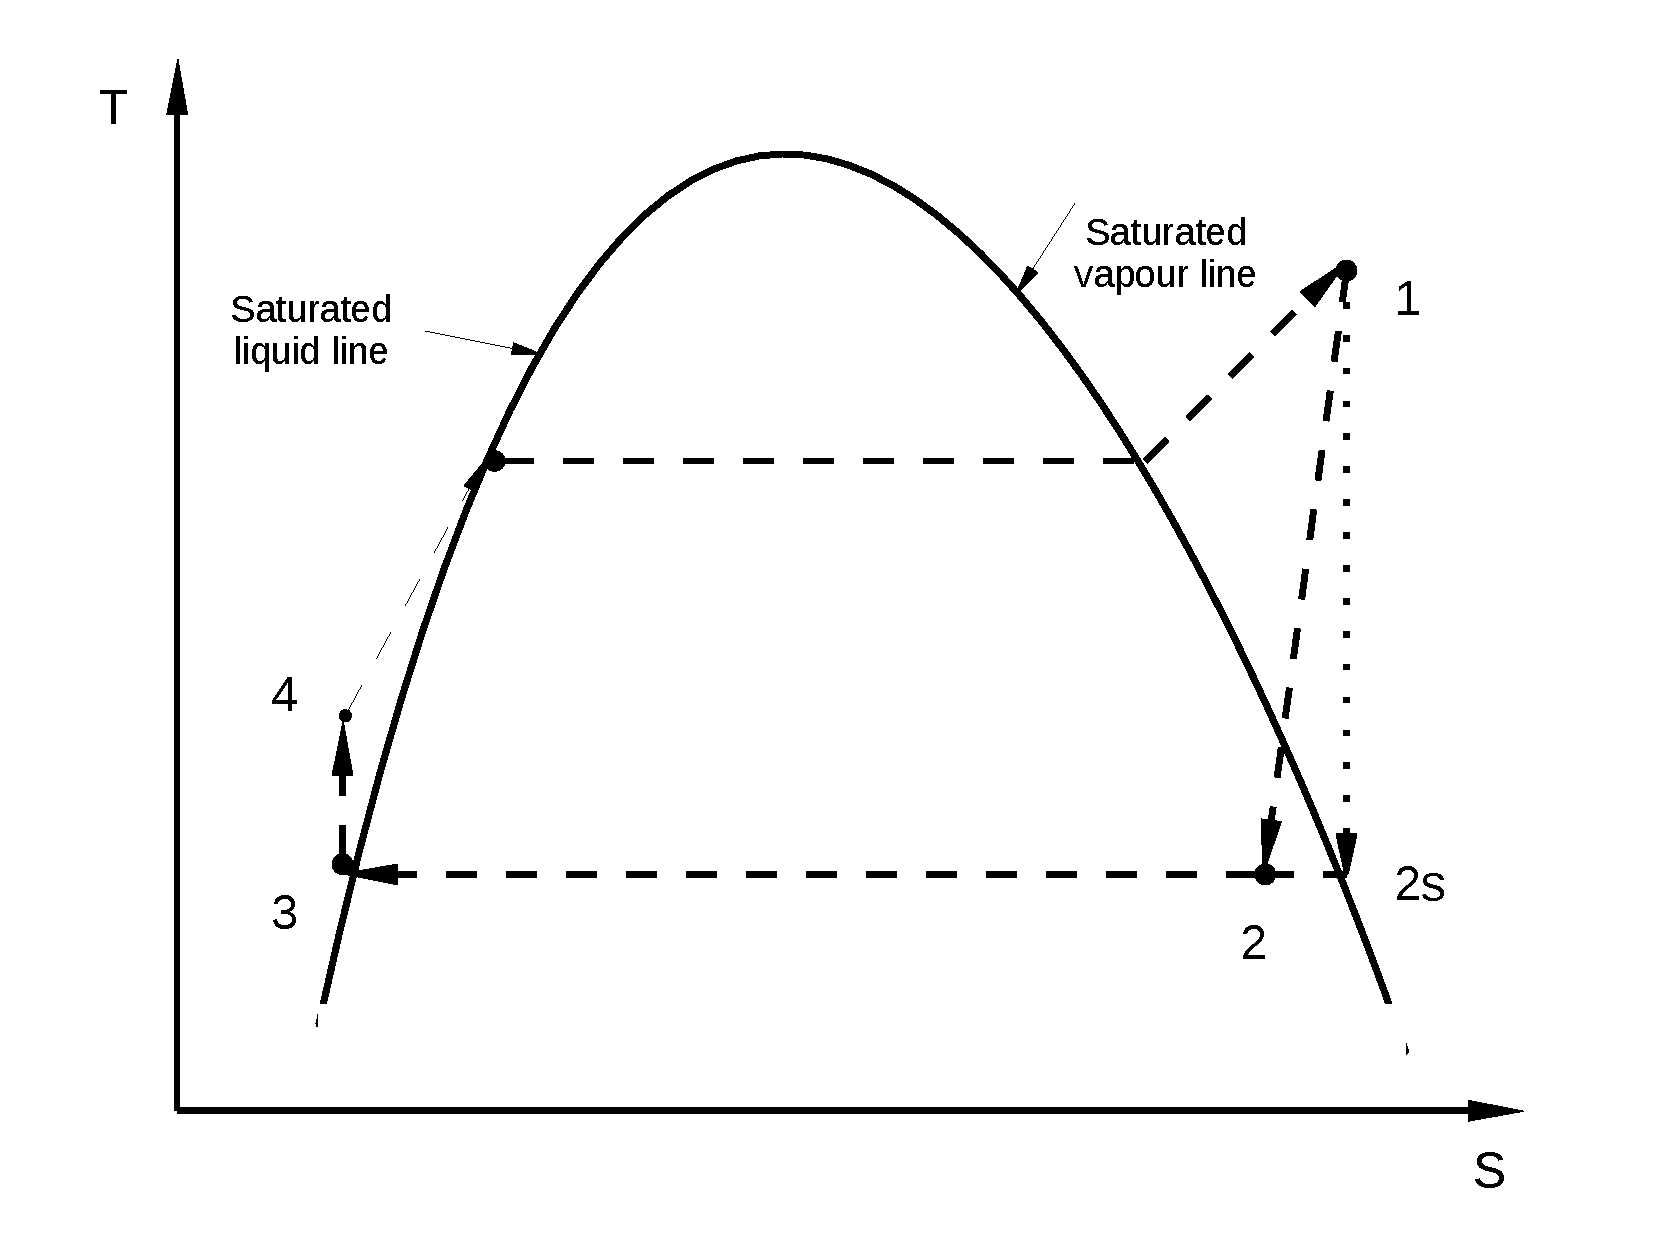
\includegraphics[width=8.cm,clip]{./Pics/TS_DIagramGeothermalBinary}
\end{center}%~\solmarks{3/3}
}
\end{enumerate} 

To solve this problem, you should assume that the saturated liquid streams are incompressible, and therefore $dH = VdP$ (where $H$, $V$ and $P$ are enthalpy, volume and pressure, respectively). Quality of the vapour is expressed as
\begin{displaymath}
x_{j} = \frc{\Psi_{j}-\Psi_{f}}{\Psi_{g}-\Psi_{f}}\;\;\;\text{with }\Psi=\left\{H,S\right\}
\end{displaymath}
where $S$ is the entropy. Efficiency of the turbine $\left(\eta_{\text{Turbine}}\right)$ and the heat exchanger $\left(\eta_{\text{HE}}\right)$ are given by,
\begin{displaymath}
\eta_{\text{Turbine}} =\frc{H_{2}-H_{1}}{H_{2s}-H_{1}} \;\;\;\text{ and }\;\;\; \eta_{\text{HE}} = \frc{\dot{Q}_{C3}}{\dot{Q_{gf}}}
\end{displaymath}
where $H_{2s}$ is the enthalpy of stream $2$ assuming ideal turbine performance (i.e., reversible expansion). $\dot{Q}_{C3}$ and $\dot{Q}_{gf}$ are the heat associated with the n-C$_{3}$ and brine streams, respectively, at the heat exchanger.

%
\end{question}

\clearpage

%%%
%%% Question 04
%%%
\begin{question}
 The excess molar volume of a solution of ethanol (1) and methyl-buthyl ether (2) at 298.15 K is given by the following expression:
\begin{displaymath}
\overline{V}^{\text{E}} =  x_{1}x_{2}\left[-1.026+0.22\left(x_{1}-x_{2}\right)\right]
\end{displaymath}
Given $\overline{V}_{1}=58.63$ cm$^{3}$.mol$^{-1}$ and $\overline{V}_{2}=118.46$ cm$^{3}$.mol$^{-1}$ $\left(\overline{V}_{i}\right.$ is the molar volume of component $i\left.\right)$.
\begin{enumerate}[(a)]
\item What is the volume of the solution when 750 cm$^{3}$ of pure ethanol is mixed with 1500 cm$^{3}$ of methyl-buthyl ether at 298.15 K?~\marks{14}
%
\solution{First, we need to calculate the number of moles $n= \frc{V}{\overline{V}}$ $\Longrightarrow$ {\bf n$_{1}$=12.79} and {\bf n$_{2}$=12.66} and the total number of moles $\left(n_{T}\right)$ is 25.455. The molar fraction can now be calculated as $x_{i}=n_{i}/n_{T}$ $\Longrightarrow$ {\bf x$_{1}$=0.5025} and {\bf x$_{2}$=0.4975}~\solmarks{4/14}. Substituting these values in,
\begin{displaymath}
{\bf \overline{V}^{\text{E}}} =  x_{1}x_{2}\left[-1.026+0.22\left(x_{1}-x_{2}\right)\right] {\bf = -0.2562 \frc{cm^{3}}{mol}}
\end{displaymath}~\solmarks{2/14}
The molar volume of the solution is given by
\begin{displaymath}
\overline{V}^{\text{E}} = \overline{V} - \sum\limits_{i=1}^{2}x_{i}\overline{V}_{i} \;\;\Longrightarrow \;\;\; {\bf \overline{V} = 88.1392\frc{cm^{3}}{mol}}
\end{displaymath}~\solmarks{2/14}
The total volume can then be calculated as 
\begin{displaymath}
{\bf V^{T}=\overline{V}.n_{T}=2243.5835\; cm^{3}}
\end{displaymath}~\solmarks{6/14} 
}
\item What would be the volume if the solution was ideal?~\marks{6}
\solution{The volume of the ideal solution is
\begin{displaymath}
{\bf V_{T}^{\text{ideal}}} = n_{T}\sum\limits_{i=1}^{2} x_{i}\overline{V}_{i} {\bf = 2250.1055\;cm^{3}}
\end{displaymath}~\solmarks{6/6}
}
\end{enumerate}
%
\end{question}

\clearpage

%%%
%%% Question 05
%%%

\begin{question}
A mixture of 2 kg of H$_{2}$ and 4 kg of N$_{2}$ was compressed in a piston-cylinder in a polytropic process with $n=1.2$. During the compression, the temperature increased from 22 to 150$^{\circ}$C. Determine the heat transfer (in {\it kJ}) and the entropy change (in $kJ/K$) of the process. The entropy change is expressed as,
\begin{displaymath}
\Delta S = m_{T}\left[\overline{C}_{v}\ln\frc{T_{2}}{T_{1}}+\frc{R}{\overline{MW}}\ln\frc{V_{2}}{V_{1}}\right] 
\end{displaymath}
where $m_{T}$ is the total mass of the gaseous mixture, $\overline{MW}$ and $\overline{C}_{v}$ are the averaged molar mass and heat capacity at constant volume of the mixture. For this range of temperature, you should assume constant heat capacity at constant volume $\left(C_{v}\right)$ of 0.745 and 10.32 kJ.(kg.K)$^{-1}$, for N$_{2}$ and H$_{2}$, respectively. Molar mass of H$_{2}$: 2.016 g.mol$^{-1}$, N$_{2}$: 28.01 g.mol$^{-1}$.~\marks{20}
\solution{For H$_{2}$ (1) and N$_{2}$ (2), n$_{1}$ = 0.9921,  n$_{2}$=0.1428 and n$_{T}$ = 1.1349 (also m$_{T}$ = 6kg) $\Longrightarrow$ ${\bf y_{1}=0.8742}$ and ${\bf y_{2}=0.1258}$~\solmarks{2/20}. Now we can calculate the averaged molecular weight $\overline{MW}$,
\begin{displaymath}
{\bf \overline{MW}} = \sum\limits_{i=1}^{2} y_{i} MW_{i} {\bf = 5.2860\frc{kg}{kgmol}} 
\end{displaymath}~\solmarks{2/20}
and
\begin{displaymath}
\overline{C}_{v}=  \sum\limits_{i=1}^{2} y_{i} C_{v,i} = 9.1155 \frc{kJ}{kg.K}
\end{displaymath}
From the first law, $dU = dQ - dW$, for the polytropic compression $\left(PV^{n}=C\right)$ we need work to be executed,
\begin{eqnarray}
dW = PdV \Longrightarrow {\bf W} &=& \int\limits_{1}^{2} P dV = \int\limits_{1}^{2} \frc{C}{V^{n}}dV = \left.\frc{CV^{1-n}}{1-n}\right|_{1}^{2}=\left.\frc{PV}{1-n}\right|_{1}^{2}=\left.\frc{n_{T}RT}{1-n}\right|_{1}^{2} \nonumber \\
                           &=& \frc{m_{T}}{\overline{MW}}\frc{R\left(T_{2}-T_{1}\right)}{1-n} {\bf = -6038.98 kJ} \nonumber
\end{eqnarray}~\solmarks{4/20}
The variation in internal energy can be calculated as,
\begin{displaymath}
{\bf \Delta U} = \sum\limits_{i=1}^{2} m_{1}C_{v,i} \Delta T {\bf = 3023.36 kJ}
\end{displaymath}~\solmarks{4/20}
Thus, the heat is 
\begin{displaymath}
{\bf Q} =\Delta U + W {\bf = -3016.62 kJ}
\end{displaymath}~\solmarks{4/20}
Now to calculate the variation in entropy,
\begin{eqnarray}
{\bf \Delta S} &=& m_{T}\left[\overline{C}_{v}\ln\frc{T_{2}}{T_{1}}+\frc{R}{\overline{MW}}\ln\frc{V_{2}}{V_{1}}\right] = m_{T}\left[\overline{C}_{v}\ln\frc{T_{2}}{T_{1}}+\frc{R}{\overline{MW}}\ln\left(\frc{T_{1}}{T_{2}}\right)^{\frc{1}{n-1}}\right]\nonumber  \nonumber \\
               &=& m_{T}\left[\overline{C}_{v}-\frc{\frc{R}{\overline{MW}}}{n-1}\right]\ln\frc{T_{2}}{T_{1}} {\bf = 2.7042 \frc{kJ}{K}}\nonumber 
\end{eqnarray}~\solmarks{4/20}
}

\end{question}

\clearpage

%%%
%%% Question 01_R
%%%
\begin{question}
\begin{enumerate}[(i)]
\item Saturated refrigerant R-134a vapour at $P_{1}=400\;kPa$ is compressed by a piston to $P_{2}=16\;\text{bar}$ in a reversible adiabatic process. Critical pressure and temperature of R-134a are 4.059 MPa and 101.06$^{\text{o}}$C.
\begin{enumerate}[(a)]
\item Calculate the work done by the piston;\marks{8}
%
\solution{In order to calculate the work executed by the piston we need to calculate the thermodynamic variables at states $1$ and $2$.
\begin{enumerate}
%
\item {\bf State 1:} Saturated vapour at $P_{1}=400$ kPa = 4 bar $\Rightarrow$ $T_{1}=T_{\text{sat}}=8.93^{\text{o}}C$, $V_{1}=V_{g}=0.0509\frc{m^{3}}{kg}$, $H_{1}=252.32\frc{kJ}{kg}$, $S_{1}=0.9145\frc{kJ}{kg.K}$ and \\
${\bf U_{1}=231.97\frc{kJ}{kg}}$~\solmarks{3/8}. 
%
\item {\bf State 2:} Adiabatic (i.e., isentropic) compression to $P_{2}=16$ bar $\Rightarrow$ $S_{2}=S_{1}=0.9145\frc{kJ}{kg.K}$. At this pressure, the saturated vapour entropy is smaller than the prescribed entropy, i.e., $S_{g}=0.8982\frc{kJ}{kg.K}<<S_{2}$. Therefore, the fluid in $2$ is at superheated state, thus (via linear interpolation): $T_{2}=61.96^{\text{o}}C<<T_{C}$, $V_{2}=0.01254\frc{m^{3}}{kg}$, $H_{2}=280.77\frc{kJ}{kg}$ and \\
${\bf U_{2}=260.71\frc{kJ}{kg}}$~\solmarks{3/8}.\\
 Notice that $P_{2} << P_{C}$ and $V_{2} << V_{1}$. 
%
\end{enumerate}
 Now, from the First Law:~\solmarks{2/8}
\begin{displaymath}
dU = dQ + dW \Rightarrow U_{2}-U_{1} = 0 + \Delta W \Rightarrow {\bf \Delta W = 28.74 \frc{kJ}{kg}}
\end{displaymath}
}
%
\item Sketch the $TS$ and $PV$ diagrams including the constant pressure and temperature lines.~\marks{4}
\solution{%Figure \ref{Ex02:Q05}. ~\solmarks{4/4}
%\begin{figure}[!h]
\begin{center}~\solmarks{4/4}
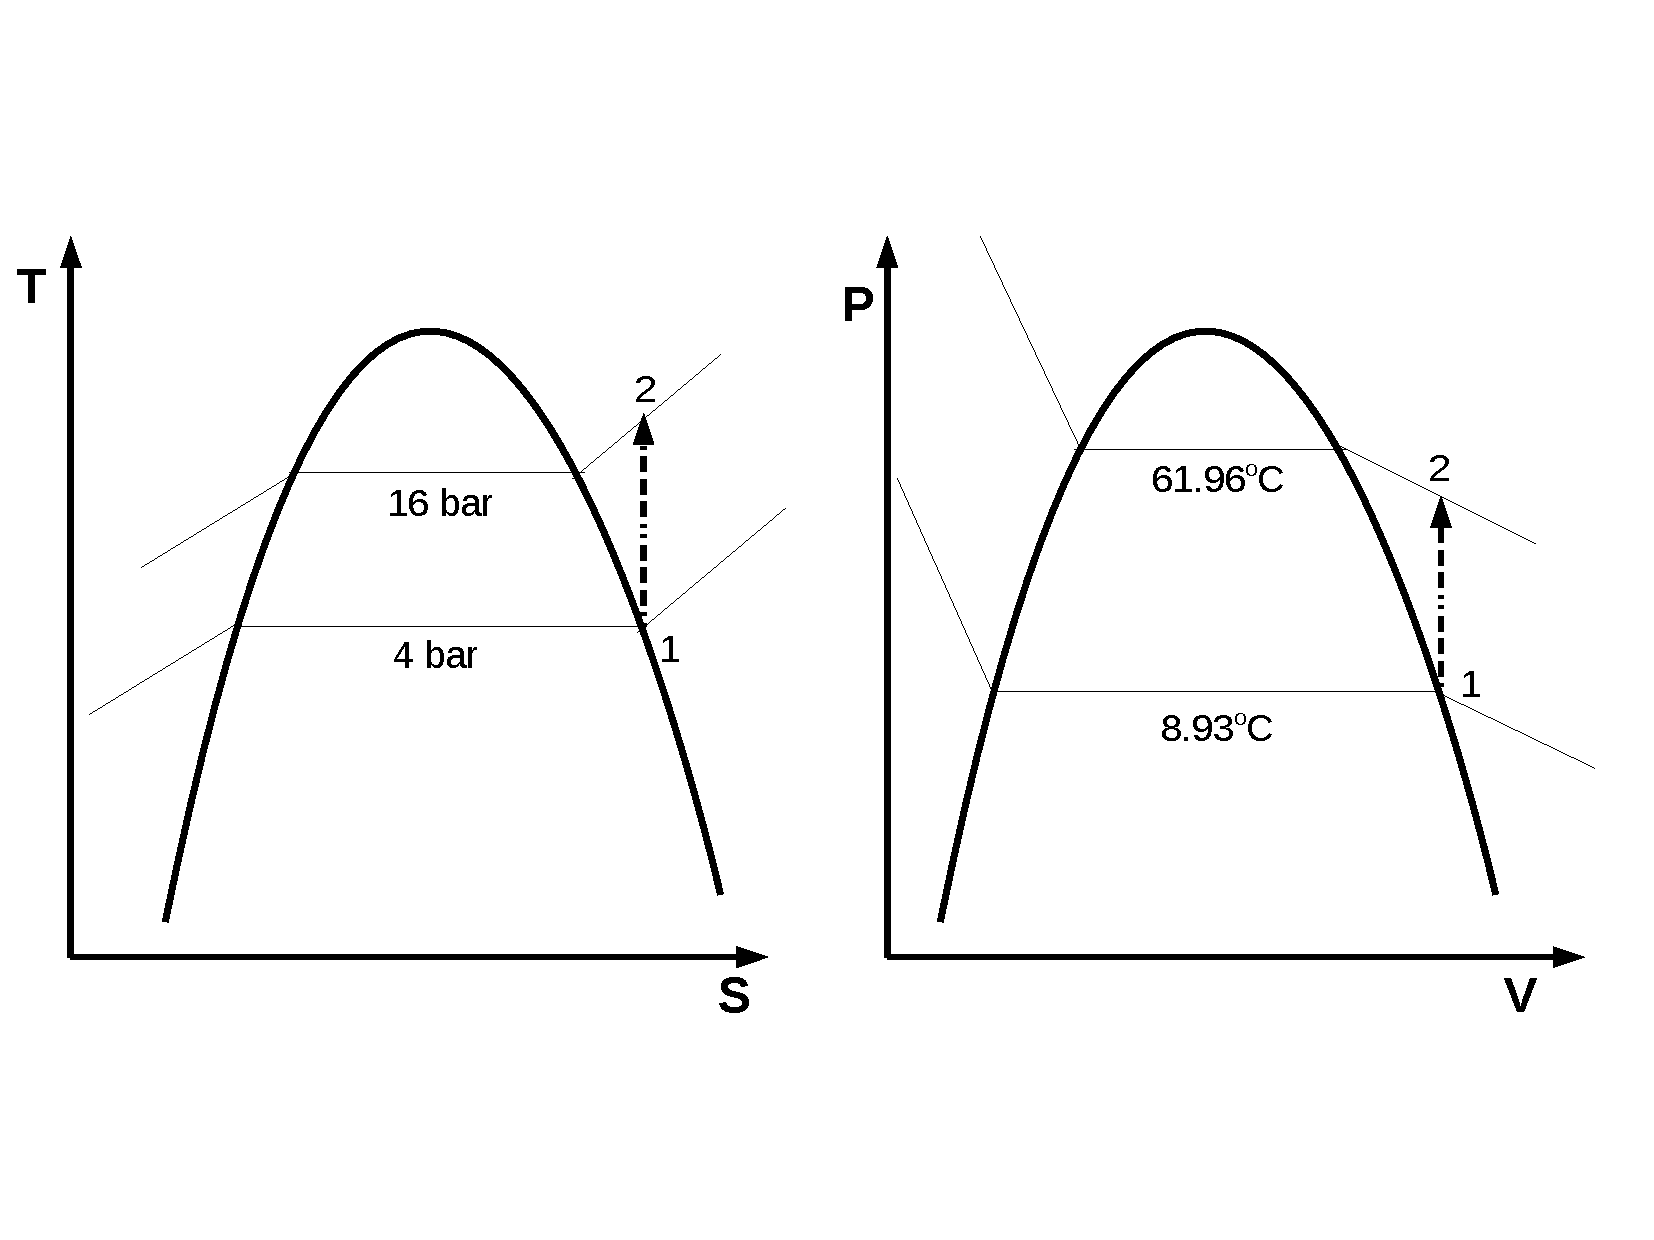
\includegraphics[width=12.0cm,height=8.0cm]{./Pics/Exam_PV-TS_Diagrams}
\end{center}
%\end{figure}
}
\end{enumerate}
%%% Saphiro 5.21 
\item A reversible power cycle receives 100 kJ by heat transfer from a hot reservoir at 327$^{\circ}$C and rejects 40 kJ by heat transfer to a cold reservoir at temperature $T_{C}$. Calculate:
\begin{enumerate}[(a)]
%
\item Thermal efficiency, $\eta_{T}\left(=\frc{W_{\text{cycle}}}{Q_{H}}\right)$, where $W_{\text{cycle}}$ is the work produced by the cycle and $Q_{H}$ is the heat associated to the hot reservoir.~\marks{4}
%
\solution{The problem supplies $Q_{H}$ = 100 kJ, $T_{H}$ = 327$^{\circ}$C and $Q_{C}$ = 40 kJ. The efficiency is given by
\begin{displaymath}
{\bf \eta_{T} } = \frc{W_{\text{cycle}}}{Q_{H}} = 1- \frc{Q_{C}}{Q_{H}} = 1 - \frc{40 kJ}{100 kJ} {\bf = 0.6} \;\; \Longrightarrow \;\; {\bf 60\%}
\end{displaymath}~\solmarks{4/4}
}  
%
\item Temperature of the cold reservoir $\left(T_{C}\right)$ in $^{\circ}$C.~\marks{4}  
%
\solution{Since the cycle operates reversibly, $\eta_{H}=\eta_{\text{max}}=1-\frc{T_{C}}{T_{H}}$. Therefore with $T_{H}$ = 327$^{\circ}$C = 600.15 K,
\begin{displaymath}
0.6 = 1 - \frc{T_{C}}{T_{H}} = 1 - \frc{T_{C}}{600.15} \;\;\Longrightarrow\;\; {\bf T_{C} = 240.06 K = -33.09^{\circ}C}
\end{displaymath}~\solmarks{4/4}
}
\end{enumerate}
%
\end{enumerate}
%
\end{question}
\clearpage



%%%
%%% Question 02
%%%
\begin{question}
\begin{enumerate}[(i)]
%
\item Derive the Maxwell relations below from the fundamental thermodynamic equations.~\marks{12}
\begin{eqnarray}
 \left(\frac{\partial T}{\partial V}\right)_{S} = -\left(\frc{\partial P}{\partial s}\right)_{V}; && 
 \left(\frc{\partial T}{\partial P}\right)_{S} = \left(\frac{\partial V}{\partial s}\right)_{P}; \nonumber \\
 \left(\frc{\partial P}{\partial T}\right)_{V} = \left(\frac{\partial S}{\partial V}\right)_{T}; &&%
  \left(\frac{\partial V}{\partial T}\right)_{P} = -\left(\frc{\partial S}{\partial P}\right)_{T} \nonumber 
\end{eqnarray}
%
\solution{First, let's assume a functional $f=f\left(a,b\right)$ and rewrite it as a function of the variables $a$ and $b$,
\begin{displaymath}
df = \left(\frc{\partial f}{\partial a}\right)_{b}da + \left(\frc{\partial f}{\partial b}\right)_{a}db
\end{displaymath}
If we define $M=\left(\frc{\partial f}{\partial a}\right)_{b}$ and $N=\left(\frc{\partial f}{\partial b}\right)_{a}$, the equation above becomes 
\begin{equation}
{\bf df = M da + N db}\label{eqn1}
\end{equation}~\solmarks{2/12}
Now, if we differentiate $M$ and $N$ with respect to $b$ and $a$, respectively,
\begin{displaymath}
\left(\frc{\partial M}{\partial b}\right)_{a} = \frc{\partial^{2} f}{\partial a\partial b}\;\;\text{ and }\;\;\left(\frc{\partial N}{\partial a}\right)_{b} = \frc{\partial^{2} f}{\partial b\partial a}
\end{displaymath}
If the functional $f$  is continuous and differentiable over all domain,
\begin{equation}\label{eqn2}
\frc{\partial^{2} f}{\partial a\partial b} = \frc{\partial^{2} f}{\partial b\partial a} \Longrightarrow {\bf \left(\frc{\partial M}{\partial b}\right)_{a} = \left(\frc{\partial N}{\partial a}\right)_{b} }
\end{equation}~\solmarks{2/12}
The fundamental thermodynamic relations, 
\begin{eqnarray}
&& dU = - PdV + TdS \nonumber \\ 
&& dH =   Tds + VdP \nonumber \\
&& dA = - PdV - SdT \nonumber \\
&& dG = - VdP - SdT \nonumber
\end{eqnarray}
have similar shape as Eqn.~\ref{eqn1}, where, for example, in the first relation: $U = f$, $M=-P$, $N=T$, $dV=da$ and $dS=db$. Using relation~\ref{eqn2}, ${\bf -\left(\frc{\partial P}{\partial S}\right)_{V}=\left(\frc{\partial T}{\partial V}\right)_{S}}$~\solmarks{2/12}. Applying the same to the remaining relations we obtain:
\begin{displaymath}
 {\bf \left(\frc{\partial T}{\partial P}\right)_{S} = \left(\frac{\partial V}{\partial s}\right)_{P}}
\end{displaymath}~\solmarks{2/12}
\begin{displaymath}
{\bf  \left(\frc{\partial P}{\partial T}\right)_{V} = \left(\frac{\partial S}{\partial V}\right)_{T}}
\end{displaymath}~\solmarks{2/12}
\begin{displaymath}
  {\bf \left(\frac{\partial V}{\partial T}\right)_{P} = -\left(\frc{\partial S}{\partial P}\right)_{T} }
\end{displaymath}~\solmarks{2/12}
}
%
\item Using the Maxwell relations above, evaluate $\left(\frc{\partial S}{\partial V}\right)_{T}$ for water vapour at 240$^{\circ}$C and specific volume of 0.4646 m$^{3}$.kg$^{-1}$ through the Redlich-Kwong equation of state,
\begin{displaymath}
P = \frc{RT}{V-b} - \frc{a}{V\left(V+b\right)T^{1/2}}
\end{displaymath}
with $a$ = 142.59 bar$\left(\frc{\text{m}^{3}}{\text{kgmol}}\right)^{2}\left(\text{K}\right)^{\frac{1}{2}}$ and $b$ = 0.0211$\frc{\text{m}^{3}}{\text{kgmol}}$.~\marks{8}
\solution{The Maxwell relation $\left(\frc{\partial P}{\partial T}\right)_{V} = \left(\frc{\partial S}{\partial V}\right)_{T}$ allows to determine $\left(\frc{\partial S}{\partial V}\right)_{T}$  from the PVT relationship in the RK EOS. Thus,
\begin{displaymath}
{\bf \left(\frc{\partial P}{\partial T}\right)_{V} = \frc{R}{V-b} + \frc{a}{2 V\left( V + b \right)T^{\frac{3}{2}}}}
\end{displaymath}~\solmarks{3/8}
Now substituting the variables by their values (and with V=0.4646 m$^{3}$.kg$^{-1}$ = 2.5811$\times$10$^{-2}$ m$^{3}$.kgmol$^{-1}$)
\begin{eqnarray}
\mathbf{\left(\frc{\partial P}{\partial T}\right)_{V}} &=& \frc{8.314\frc{kJ}{kgmol.K}}{\left(2.5811\times 10^{-2} - 0.0211\right) \frc{m^{3}}{kgmol}} + \nonumber \\
&& \frc{ 142.59\; bar\left(\frc{m^{3}}{kgmol}\right)^{2}.K^{1/2}} {2 \times 2.5811\times 10^{-2} \frc{m^{3}}{kgmol} \left( 2.5811\times 10^{-2} + 0.0211 \right) \frc{m^{3}}{kgmol} \left(513.15 K\right)^{3/2} } \nonumber  \\
&=& \mathbf{\left(\frc{\partial S}{\partial V}\right)_{T}} = \mathbf{2271.30\;\frc{kJ}{m^{3}.K}}\nonumber 
\end{eqnarray}~\solmarks{5/8}

}
%
\end{enumerate}
\end{question}
\clearpage

%%%
%%% Question 03
%%%
\begin{question}
The steam generator of a nuclear power plant produces 25 kg.s$^{-1}$ of water-steam at P$_{1}$ = 140 bar and T$_{1}$= 415$^{\circ}$C. The fluid is used to drive a turbine (isentropic expansion) producing power $\left(W_{T}\right)$ at P$_{2}$ = 2.5 bar. Before the vaporisation in the boiler, the fluid needs to be condensed into liquid water (stage 3) producing $Q_{C}$ of heat. 
\begin{center}
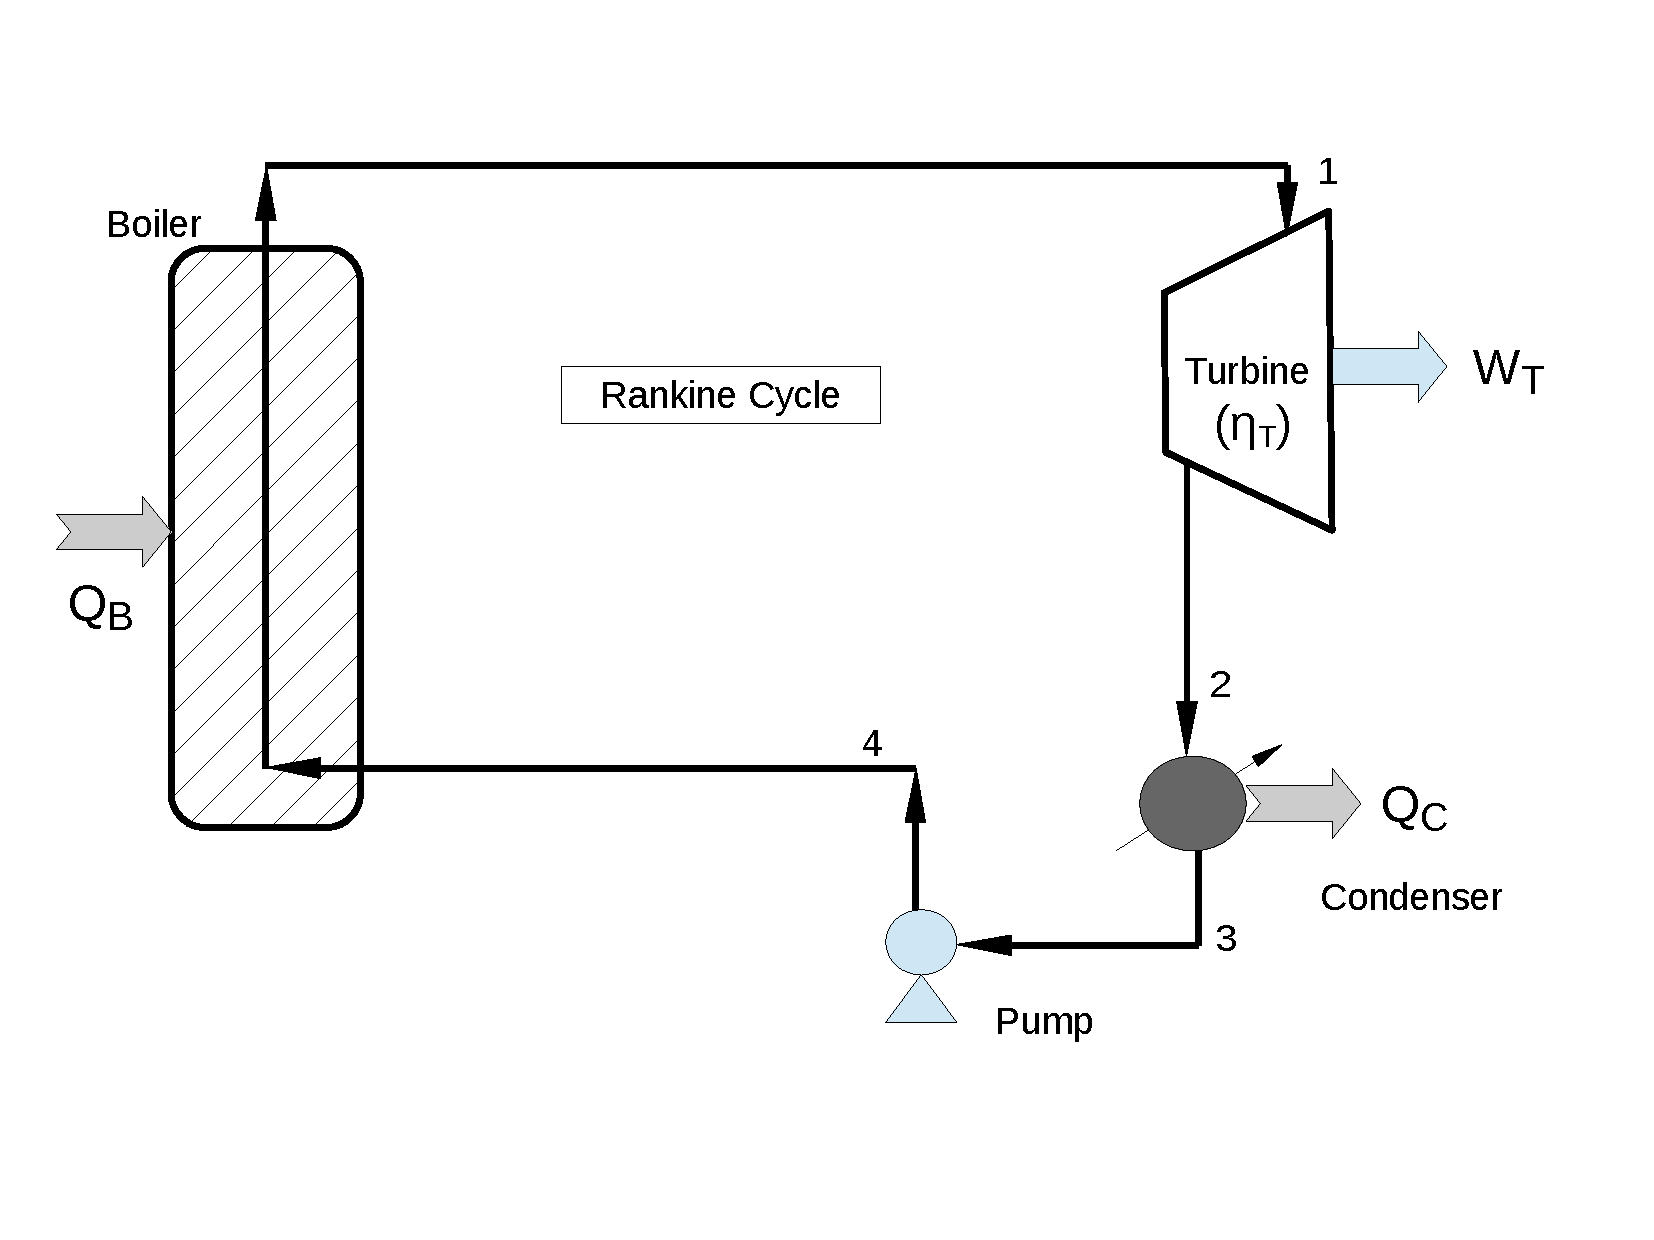
\includegraphics[width=10.cm,height=8.cm,clip]{./Pics/RankineCycle2}
%\caption{ Reheat and regenerative Rankine cycle with 2 turbines.}
\label{exam_mod02_rankinecycle}
\end{center}
\begin{enumerate}[(a)]
\item Calculate $H_{1}, H_{2}, H_{4}, S_{1} \text{ and } x_{2}$ (quality of the steam).~\marks{10}
%
\solution{\begin{description}
\item[State 1:] At P$_{1}$ = 140 bar, T$_{sat}$ = 336.75$^{\circ}$C $>$ T$_{1}$= 415$^{\circ}$C, therefore the fluid is at superheated state. From the superheated steam table (via linear interpolation), {\bf H$_{1}$ = 3054.51 kJ.kg$^{-1}$}~\solmarks{2/10} and \\
{\bf S$_{1}$ = 6.0208 kJ.(kg.K)$^{-1}$}~\solmarks{2/10}.
\item[State 2:] Isentropic expansion at P$_{2}$ = 2.5 bar $\longrightarrow$ S$_{2}$=S$_{1}$. We can calculate the quality of the water-steam at 2.5 bar,
\begin{displaymath}
{\bf x_{2}} = \frc{S_{2}-S_{f}}{S_{g}-S_{f}} {\bf = 0.8105} 
\end{displaymath}~\solmarks{2/10}
With the quality we can then calculate the H$_{2}$,
\begin{displaymath}
x_{2} = \frc{H_{2}-H_{f}}{H_{g}-H_{f}} \;\;\Longrightarrow \;\; {\bf H_{2} = 2303.50\frc{kJ}{kg}} 
\end{displaymath}~\solmarks{2/10}
\item[State 3:] After the condenser, water is at liquid state at P$_{3}$=P$_{2}$ (no pressure drop) with H$_{3}$ = H$_{f}$ = 535.37 kJ.kg$^{-1}$, S$_{3}$ = S$_{f}$ = 1.6072 kJ.(kg.K)$^{-1}$ and V$_{3}$ = V$_{f}$ = 1.0672$\times$10$^{-3}$ m$^{3}$.kg$^{-1}$.
\item[State 4:] Assuming the liquid water is incompressible $dH\equiv VdP$ with P$_{4}$ = P$_{1}$
\begin{displaymath}
{\bf H_{4}} = H_{3} + V_{3}\left(P_{4} - P_{3}\right) = {\bf 550.04 \frc{kJ}{kg}}
\end{displaymath}~\solmarks{2/10}
\end{description}
}
%
\item Determine the power produced in the turbine $\left(W_{T}\right)$ in MW.~\marks{2}
%
\solution{For $\dot{m}_{w}$ = 25 kg.s$^{-1}$,
\begin{displaymath}
{\bf W_{T}} = \dot{m}_{w}\left(H_{1}-H_{2}\right) {\bf = 18775.25\frc{kJ}{s} = 18.8 MW}
\end{displaymath}~\solmarks{2/2}
}
%
\item Determine the heat extracted from the steam $\left(Q_{C}\right)$ in MW.~\marks{2}
%
\solution{\begin{displaymath}
{\bf Q_{C} }= \dot{m}_{w}\left(H_{2}-H_{3}\right) {\bf = 44203.25\frc{kJ}{s} = 44.2 MW}
\end{displaymath}~\solmarks{2/2}
}
\item Determine the heat supplied by the boiler $\left(Q_{B}\right)$ in MW.~\marks{2}
%
\solution{\begin{displaymath} 
{\bf Q_{B}} = \dot{m}_{w}\left(H_{1}-H_{4}\right) {\bf = 62611.75\frc{kJ}{s} = 62.6 MW}
\end{displaymath}~\solmarks{2/2}
}
%
\item Calculate the efficiency of the cycle $\left(\eta_{\text{cycle}}=\frac{W_{T}}{Q_{B}}\right)$.~\marks{2}
%
\solution{\begin{displaymath}
{\bf \eta_{\text{cycle}} } =  \frc{W_{T}}{Q_{B}} {\bf = 0.30} \Longrightarrow {\bf 30\%}
\end{displaymath}~\solmarks{2/2}
}
%
\item Sketch the temperature $\times$ entropy (TS) diagram for the process indicating the liquid and vapour saturated lines and each stage of the water-steam Rankine cycle.~\marks{2}
\solution{~\solmarks{2/2}
\begin{center}
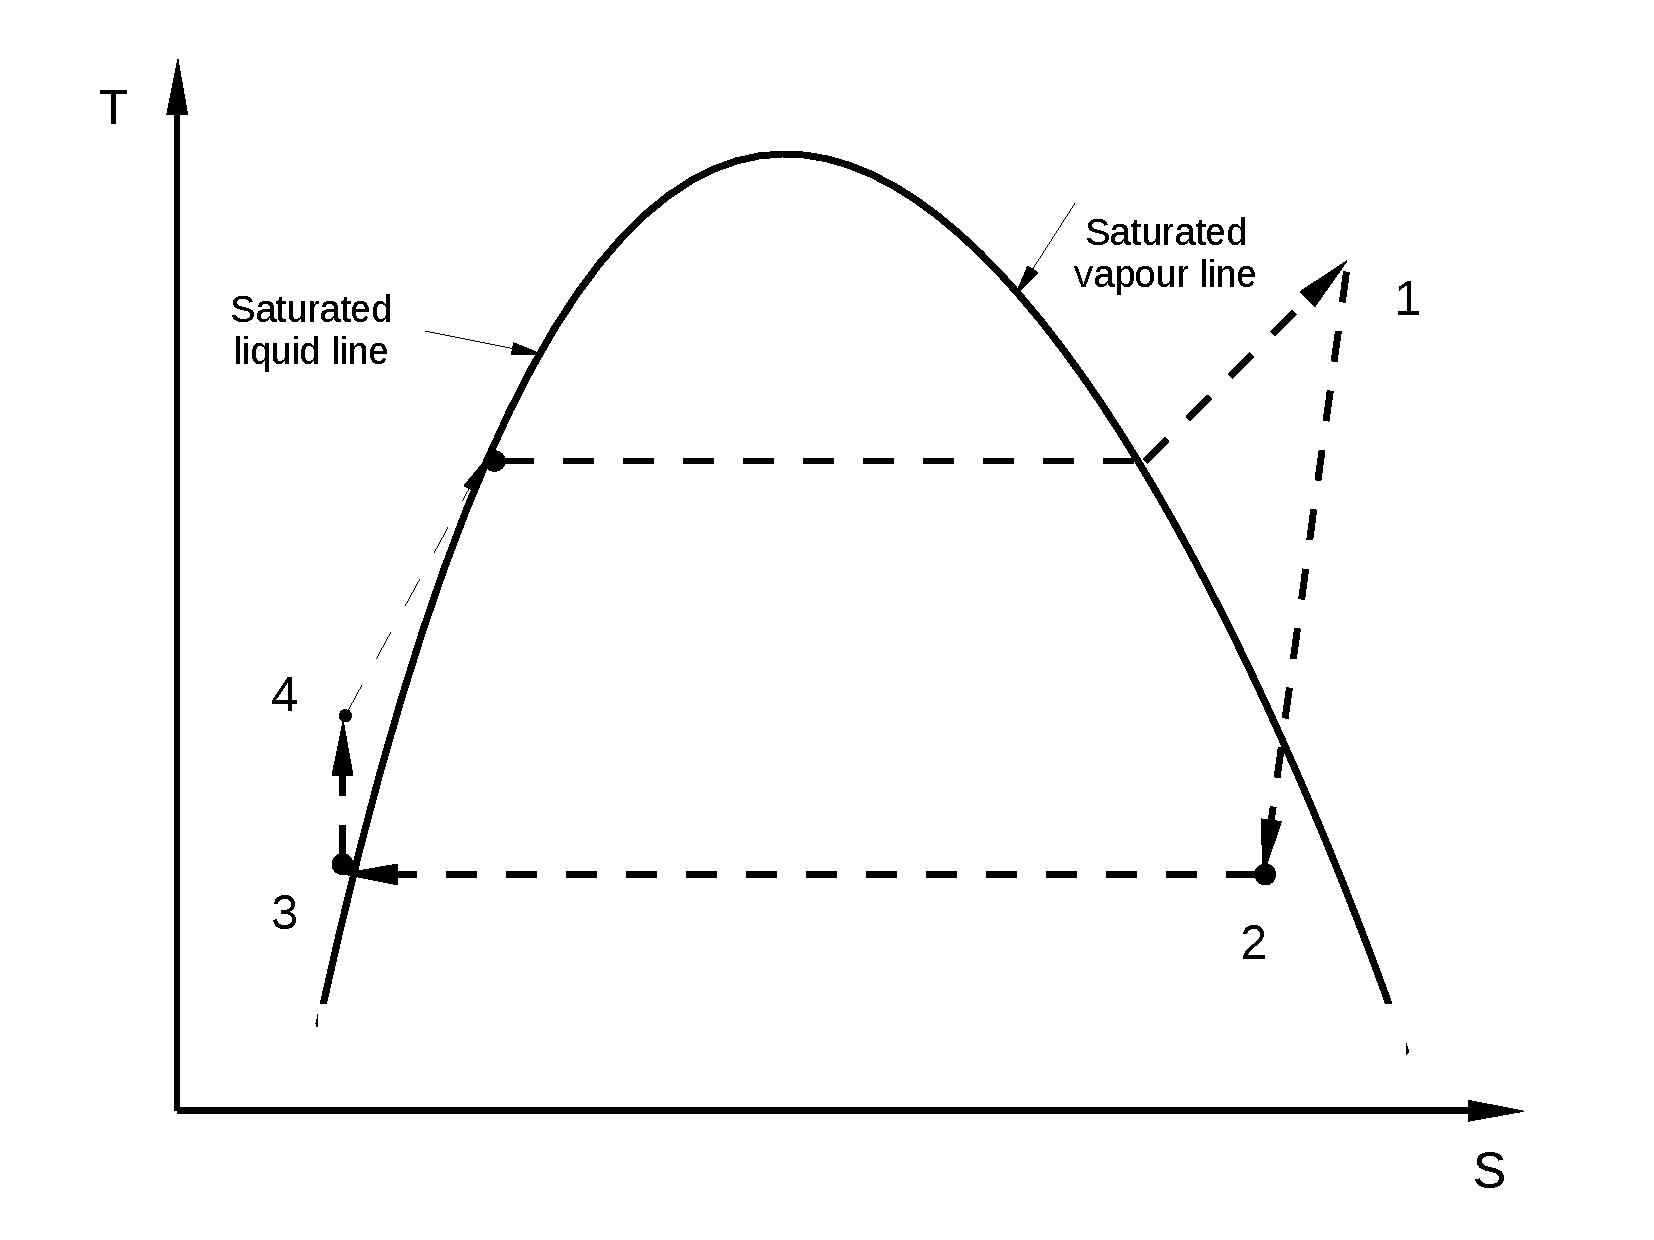
\includegraphics[width=8.cm,clip]{./Pics/TS_DIagramExam2}
\end{center}%~\solmarks{3/3}
}
\end{enumerate}
To solve this problem, you should assume that the saturated liquid streams are incompressible, and therefore $dH = VdP$ (where $H$, $V$ and $P$ are enthalpy, volume and pressure, respectively). Quality of the vapour is expressed as
\begin{displaymath}
x_{j} = \frc{\Psi_{j}-\Psi_{f}}{\Psi_{g}-\Psi_{f}}\;\;\;\text{with }\Psi=\left\{H,S\right\}
\end{displaymath}
where $S$ is the entropy. 

\end{question}
\clearpage

%%%
%%% QUESTION 4 (SM&VN 12.26)
%%%
\begin{question}
Two chemical species, $1$ and $2$ are mixed in a solution at 25$^{\circ}$C and atmospheric pressure. The volume change is given by the following equation,
\begin{displaymath}
\Delta V = x_{1}x_{2}\left(45 x_{1} +  25x_{2}\right)
\end{displaymath} 
where $\Delta V$ is expressed in cm$^{3}$.gmol$^{-1}$. At these temperature and pressure conditions, V$_{1}$ = 110 and V$_{2}$ = 90 cm$^{3}$.gmol$^{-1}$. Determine the partial molar volumes of the chemical species in a solution containing 40$\%$-mol of species $1$.~\marks{20}
\solution{ $x_{1} = 0.4$ and $x_{2}=1-x_{1}=0.6$.  The volume change is the excess volume,
\begin{displaymath}
\Delta V = x_{1}x_{2}\left(45 x_{1} +  25x_{2}\right) = {\bf V^{\text{E}} = 7.92\frc{cm^{3}}{gmol}}
\end{displaymath}~\solmarks{5/20}
The volume of the binary solution is given by
\begin{displaymath}
{\bf V} = V^{\text{E}} + x_{1}V_{1}+x_{2}V_{2} {\bf = 105.92 \frc{cm^{3}}{gmol}}
\end{displaymath}~\solmarks{5/20}
The partial molar properties in binary mixtures can be obtained by $\overline{M}_{1} = M + x_{2}\frc{d M}{dx_{1}}$ and $\overline{M}_{2} = M - x_{1}\frc{d M}{dx_{1}}$, thus for partial molar volumes
\begin{displaymath}
{\bf \overline{V}_{1}} = V + x_{2} \frc{d V}{dx_{1}} {\bf = 124.76 \frc{cm^{3}}{gmol}}
\end{displaymath}~\solmarks{3/20}
and
\begin{displaymath}
  {\bf \overline{V}_{2}} = V - x_{1} \frc{d V}{dx_{1}} {\bf = 93.36 \frc{cm^{3}}{gmol}}
\end{displaymath}~\solmarks{3/20}
where
\begin{eqnarray}
V &=& V^{\text{E}} + \sum\limits_{i=1}^{n}x_{i}V_{i}  = x_{1}x_{2}\left(45x_{1}+25x_{2}\right)+x_{1}V_{1}+x_{2}V_{2}  \nonumber \\
  &=&  x_{1}\left(1-x_{1}\right)\left[45x_{1}+25\left(1-x_{1}\right)\right]+x_{1}V_{1}+\left(1-x_{1}\right)V_{2} \nonumber
\end{eqnarray}
and
\begin{displaymath}
\mathbf{\frc{dV}{dx_{1}} = 25 -10x_{1}-60x_{1}^{2} + \left(V_{1}-V_{2}\right)}
\end{displaymath}~\solmarks{4/20}

We can verify the solution through
\begin{displaymath}
V = x_{1}\overline{V}_{1}+x_{2}\overline{V}_{2}=105.92 \frc{cm^{3}}{gmol}
\end{displaymath}
}
\end{question}

\clearpage

%%%
%%% QUESTION 5
%%%
\begin{question}
\begin{enumerate}[(i)]
% SM&VN 10.13
\item A concentrated binary solution containing mainly species $2$ $\left(\text{though } x_{2}\not= 1\right)$ is in equilibrium with a vapour phase containing both species $1$ and $2$. Pressure and temperature of this two-phase system are 1 bar and 298.15 K. Given $\mathcal{H}_{1}$ = 200 bar (Henry constant) and P$_{2}^{\text{sat}}$ = 0.10 bar, calculate $x_{1}$ and $y_{1}$.~\marks{10/10}
%
\solution{Assuming that at 1 bar the vapour phase behaves as an ideal gas. The vapour phases fugacities are then equal to the partial pressures. Assume the Lewis/Randall rule applies to concentrated species $2$ and that Henry's law applies to dilute species $1$, therefore,
\begin{displaymath}
y_{1}P=\mathcal{H}_{1}x_{1};\;\;\text{ and }\;\; y_{2}P= x_{2}P_{2}^{\text{sat}}
\end{displaymath}
with $x_{1}+x_{2}=1$. Thus $P = y_{1}P + y_{2}P$ becomes,~\solmarks{5/10}
\begin{displaymath}
P = \mathcal{H}_{1}x_{1}+\left(1-x_{1}\right)P_{2}^{\text{sat}} \;\;\Longrightarrow {\bf x_{1} = 4.502\times 10^{-3}}
\end{displaymath}
and ${\bf y_{1}=\frc{\mathcal{H}_{1}x_{1}}{P}=0.9}$.~\solmarks{5/10}
}
%
% SM&VN 10.19
\item Chemical species $A$ and $B$ are in vapour-liquid equilibrium at 298.15 K. The following conditions are applied to this system:\begin{center}
\begin{tabular}{l l}
$\ln\gamma_{A} = 1.8x_{B}^{2}$ & $\ln\gamma_{B}=1.8x_{A}^{2}$ \\
$P_{A}^{\text{sat}}$ = 1.24 bar & $P_{B}^{\text{sat}}$ = 0.89 bar
\end{tabular} 
\end{center}
Assuming that $y_{i}P = x_{i}\gamma_{i}P_{i}^{\text{sat}}$ (where $\gamma_{i}$ is the activity coefficient of species $i$) is valid, 
\begin{enumerate}[(a)]
\item Calculate the pressure $P$ and the vapour mole fraction $y_{A}$ for a liquid mole fraction $x_{A}=0.65$.~\marks{6}
%
\solution{With $x_{A}$ =0.65 and $x_{B}$=0.35, we can calculate the activity coefficients, $\gamma_{A}$ $\gamma_{B}$ and apply in $P = x_{A}\gamma_{A} P_{A}^{\text{sat}} + x_{B}\gamma_{B} P_{B}^{\text{sat}}$ leading to {\bf P=1.671 bar}~\solmarks{3/6}. The vapour mole fraction is obtained from $y_{A} = \frc{x_{A}\gamma_{A}P_{A}^{\text{sat}}}{P}$, leading to  ${\bf y_{A}=0.6013}$.~\solmarks{3/6} 
} 
%
\item Calculate the range of overall mole fraction $z_{A}$ in which this system may exist.~\marks{4}
\solution{From mass balance for species $A$~\solmarks{1/4}
\begin{displaymath}
z_{A} = V y_{A} + L x_{A} \Longrightarrow z_{A} =V y_{A} + (1-V)x_{A} \Longrightarrow {\bf V= \frc{z_{A}-x_{A}}{y_{A}-x_{A}}}
\end{displaymath}
The overall vapour mole fraction $V$, varies from 0 to 1, ${\bf 0\leq V\leq 1}$~\solmarks{1/4}, therefore (replacing in the equation above) ${\bf 0.6013\leq z_{A} \leq 0.65}$.~\solmarks{2/4}
}
\end{enumerate}

\end{enumerate}

\end{question}



\vfill
\paperend

\begin{comment}

\clearpage

\begin{center}
\Large{List of Equations}
\end{center}

\begin{itemize}
%%%
\item Generic cubic equation of state:
\begin{eqnarray}
&& Z= 1 + \beta - q\beta \frc{Z - \beta} {\left(Z+\varepsilon\beta\right)\left(Z+\sigma\beta\right)}  \;\;\text{(vapour and vapour-like roots)}\nonumber\\
&& Z= 1 + \beta + \left(Z + \epsilon\beta\right)\left(Z+\sigma\beta\right)\left(\frc{1+\beta-Z}{q\beta}\right)  \;\;\text{(liquid and liquid-like roots)}\nonumber\\
&& \text{with }\; \beta=\Omega\frc{P_{r}}{T_{r}} \;\;\text{ and } \;\; q=\frc{\Psi\alpha\left(T_{r}\right)}{\Omega T_{r}}  \nonumber \\
&&\alpha_{\text{SRK}} = \left[ 1 + \left( 0.480 + 1.574 \omega - 0.176\omega^{2}\right)\left(1-\sqrt{T_{r}}\right)\right]^{2}  \nonumber \\
&&\alpha_{\text{PR}} = \left[ 1 + \left( 0.37464 + 1.54226 \omega - 0.26992\omega^{2}\right)\left(1-\sqrt{T_{r}}\right)\right]^{2} \nonumber
\end{eqnarray} 
    \begin{center}
       \begin{tabular}{| l | c c c c c| }
       \hline
          {\bf EOS}  & {\bf $\alpha$} & {\bf $\sigma$}  & {\bf $\varepsilon$} & {\bf $\Omega$} & {\bf $\Psi$ } \\
       \hline
            vdW      & 1              & 0               & 0                  & 1/8            & 27/64          \\
            RK       & T$_{r}^{-1/2}$  & 1                & 0                  & 0.08664       & 0.42748        \\
           SRK       &$\alpha_{\text{SRK}}$& 1            & 0                   & 0.08664       & 0.42748        \\
            PR       &$\alpha_{\text{PR}}$& 1+$\sqrt{2}$   & 1-$\sqrt{2}$        & 0.07780        & 0.45724  \\
       \hline
       \end{tabular}
    \end{center}

%%%
\item Newton-Raphson (root-finder) method: $X_{i} = X_{i-1} - \frc{\mathcal{F}\left(X_{i-1}\right)}{d\mathcal{F}/dX\left(X_{i-1}\right)}$

%%%
\item Fundamental thermodynamic equations:\\
\begin{tabular}{c c c c}
$dU = dQ + dW$;  & $dH = dU + d(PV)$; & $dA = dU -d(TS)$; & $dG=dH-d(TS)$ \\
$dU = TdS - PdV$;& $dH = TdS + VdP$;  & $dA = -SdT - PdV$;& $dG = -SdT + VdP$ \\ 
\end{tabular}\\
\begin{tabular} {c c}
$dH = C_{p}dT + \left[ V - T\left(\frc{\partial V}{\partial T}\right)_{P}\right]dP$; &  $dS=C_{p}\frc{dT}{T} - \left(\frc{\partial V}{\partial T}\right)_{P}dP$ \\
$dU = C_{v}dT + \left[T\left(\frc{\partial P}{\partial T}\right)_{V} - P\right]dV$;  & $dS = C_{v}\frc{dT}{T} - \left(\frc{\partial P}{\partial T}\right)_{V}dV$
\end{tabular}

%%% 
\item Polytropic Relations:\\
\begin{displaymath} 
\frc{T_{2}}{T_{1}} =\left(\frc{P_{2}}{P_{1}}\right)^{\frac{\gamma-1}{\gamma}} = \left(\frc{V_{1}}{V_{2}}\right)^{\gamma-1}\;\; ; 
TV^{\gamma-1} =\text{ const};\; TP^{\frac{1-\gamma}{\gamma}}=\text{ const};\; PV^{\gamma}=\text{ const} 
\end{displaymath}

%%%
\item Raoult's Law:\\
\begin{displaymath}
y_{i}P = x_{i}P_{i}^{\text{sat}}\;\;\;\text{ and } \;\;\; y_{i}P = x_{i}\gamma_{i}P_{i}^{\text{sat}}\;\;\;\text{ with } i=1,2,\cdots N
\end{displaymath}

%%%
\item Henry's Law:\\
\begin{displaymath}
x_{i}\mathcal{H}_{i} = y_{i}P\;\;\;\text{ with } i=1,2,\cdots N
\end{displaymath}

%%%
\item Antoine Equation:\\
\begin{displaymath}
\log_{10} P^{\star} = A-\frc{B}{T+C}\;\;\;\text{ with P}^{\star}\text{ in mm-Hg and T in }^{\circ}\text{C}
\end{displaymath}

%%%
\item Solutions:\\
\begin{displaymath}
M^{\text{E}} = M - \sum\limits_{i=1}^{N} x_{i}M_{i}; \; \overline{M}_{1}=M+x_{2}\frc{d M}{dx_{1}};\; \overline{M}_{2} = M - x_{1}\frc{d M}{dx_{1}}
\end{displaymath}

\end{itemize}


\vfill 

{
  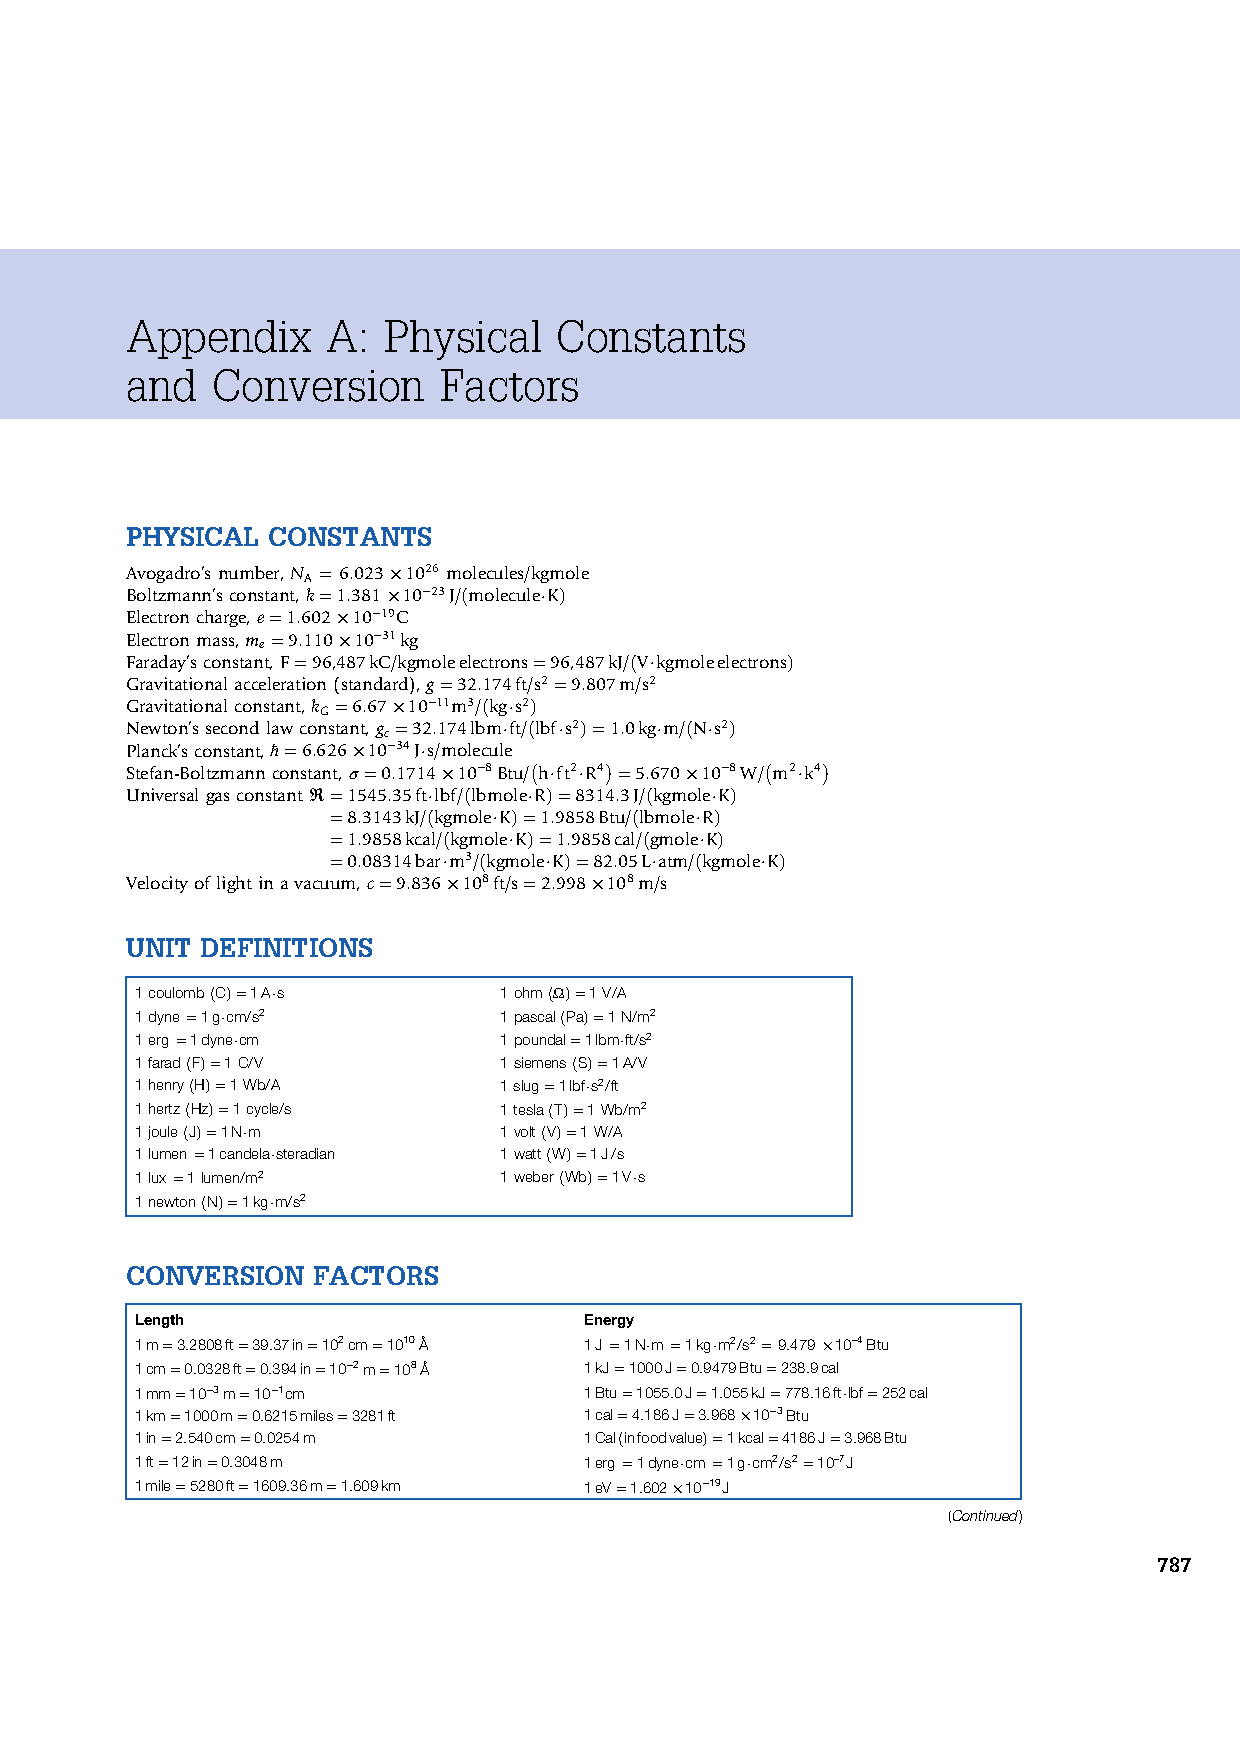
\includepdf[pages=-,fitpaper]{./Pics/ChemEng_UnitConv}
  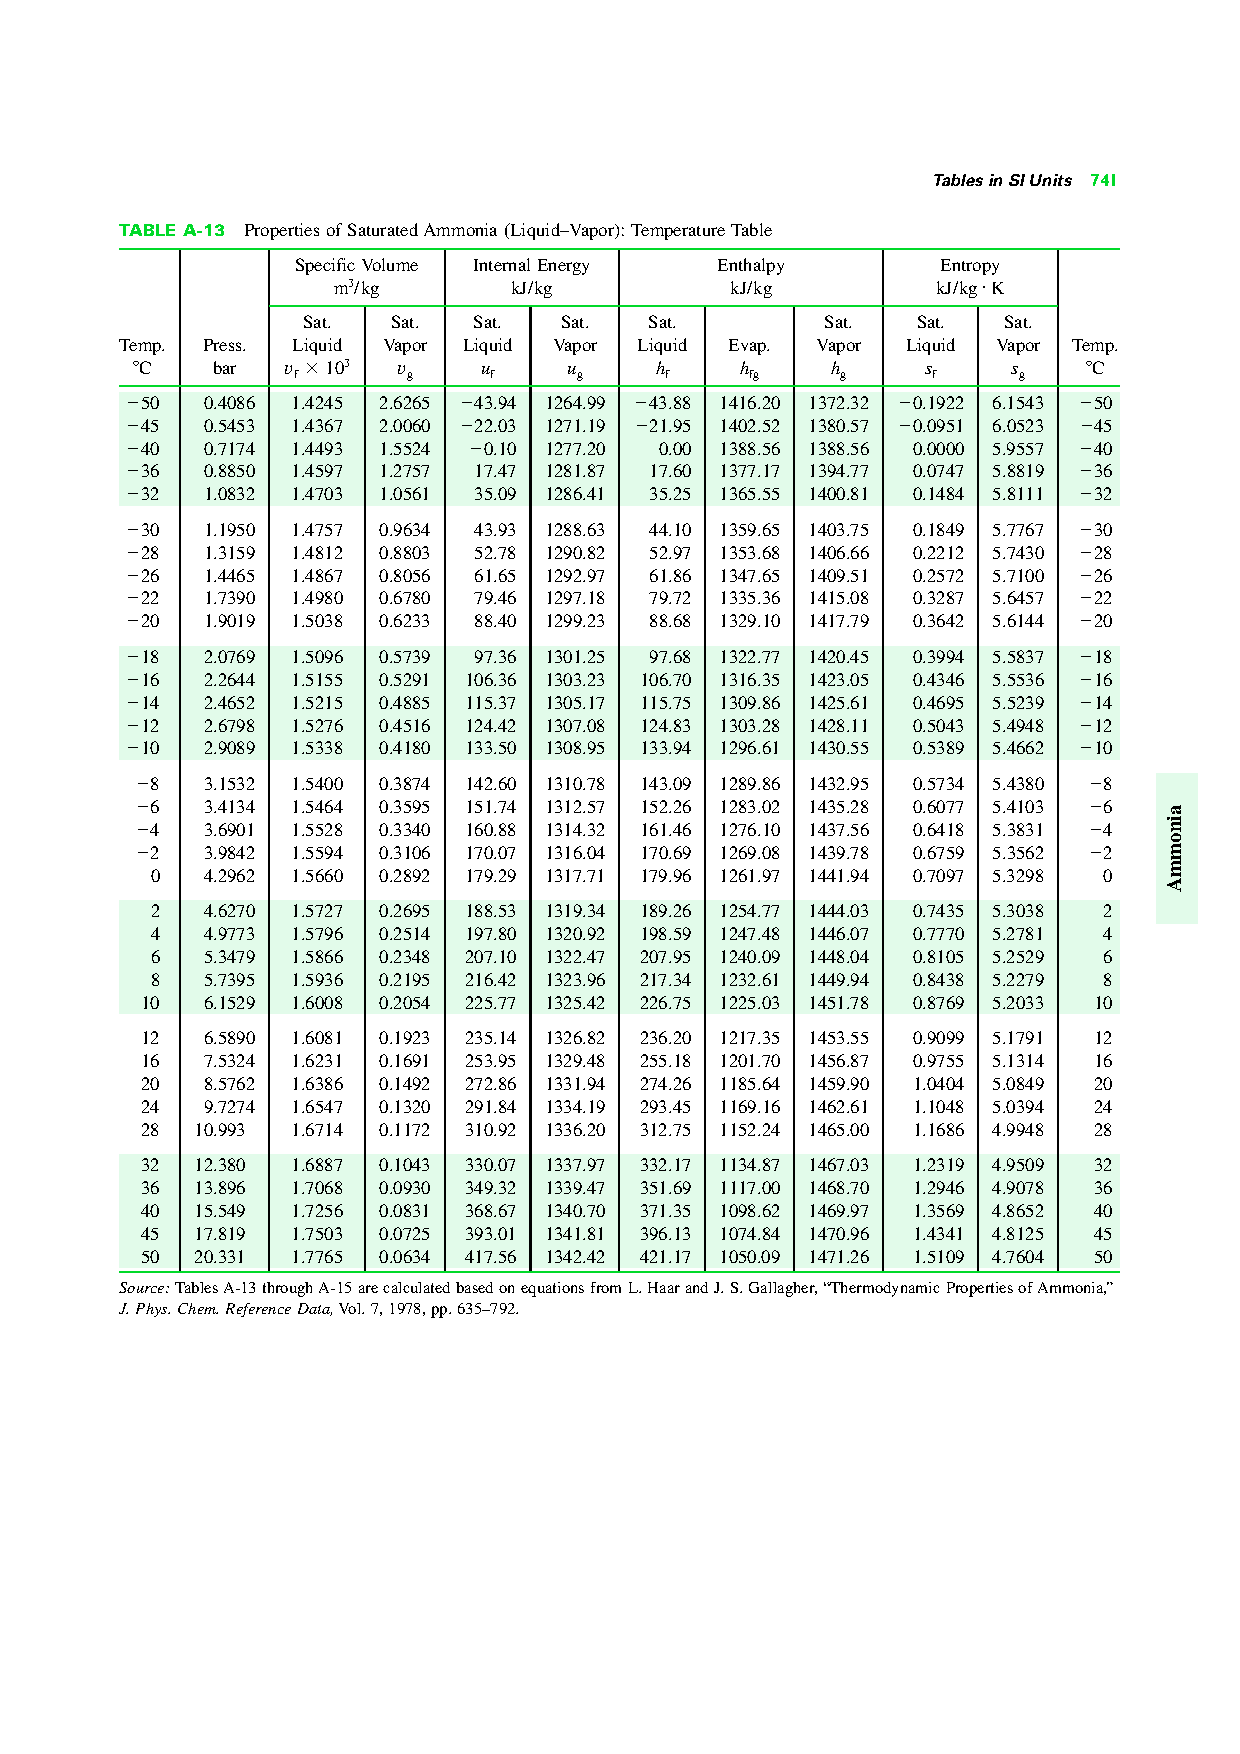
\includepdf[pages=-,fitpaper]{./Pics/ChemEng_NH3Tables}
}

\end{comment}

\end{document}
